\documentclass{article}
\usepackage[margin=0.8in]{geometry}
\usepackage{amsmath, amssymb, bm, enumitem, hyperref}
\usepackage{graphicx}

\title{Control of Nonlinear Spacecraft Attitude Motion}
\date{}

\setlength{\parskip}{5pt}

\begin{document}
\maketitle
Last compiled: \today

\newpage
\section*{Preface}
\newpage

\tableofcontents

\newpage
\section{Introduction}
\subsection{Course introduction}
This course is about nonlinear spacecraft attitude control. In previous two courses, we understood the motion and derived nonlinear equations of motion for rigid bodies. Now we want to answer the question on how to apply feedback control strategy to achieve desired orientation or tumble rate for that dynamics. We will tackle both regulation and tracking problems.

Particular challenges that we encounter in our journey of nonlinear control design are:
\begin{enumerate}
  \item What is a nonlinear stability?
  \item Which mathematical tool allows us to design control law that guarantees stability?
  \item If the control law is stable does it actually converge? (Do stability imply convergence?)
  \item If it converge, is it robust to unmodeled perturbations?
\end{enumerate}

Finally, we will discuss different control implementations that deal with saturations and gain designs. Stability is always nice for control law, but would not want  our control to converge after six years when we want it to be in six days. This is why it is important to study how gain impacts the performance of control system. Similarly, we will look at different implementations of saturation for limited actuation capability and apply it to a system with reaction wheels. This helps us to have perfect linear closed loop dynamics. 

\subsection{Overview of the course}

\subsubsection*{Stability}
Control, to me, is a way to take dynamics of the system which nature (physics) gave us and modify it to put it in a form that now makes it a stable system. For example, a simple pendulum when inverted is an unstable system. We can, however, use suitable motor actuated system to balance the inverted pendulum in its upright position which is robust to certain magnitude of perturbations. Here, we used actuators to alter the nature of the pendulum and made it a stable system. We are using the term \textit{stable} quite candidly, but what does stability actually mean? That we are going to explore and we will see how the notion of stability for nonlinear system contrasts to that of linear dynamical system.

\subsubsection*{Nonlinear control}
I have a lot of argument with my colleagues and they are like, ``Ah! but our control is linear and look I can guarantee all these things which are better.'' I know yes, but there is a problem with such statements. Life is not linear. The equations for kinematics and kinetics of spacecraft are cross coupled and really a nonlinear system. It is true, we can linearize the equations and it opens all the linear analysis tools that can be used for spacecraft control. But there is a problem with this approach, linearization does not confirm the global performance of the control. This is because linearization is performed about some point in the space space and the stability argument which follows applies around that point only. It is only with the analytical tool of nonlinear control design that we can guarantee the stability, if at all, of the nonlinear dynamics. It is this nonlinear control design what we are dealing with in the course.

\subsubsection*{Control problems}
We will be dealing with the control laws for regulation and tracking problems. 
In the \textit{regulation problem}, we define an inertial frame such that it aligns with the orientation we want to achieve. Now, with respect to that inertial frame, we are trying to achieve the desired equilibrium orientation by driving all the states to zero (i.e. we are trying to align the body frame to the new inertial frame). An example is Hubble space telescope having to correct its orientation to point its telescope towards Andromeda galaxy. Once the body frame is aligned with the virtual inertial frame we created by driving all the states to zero, attitude control mission is complete.

The \textit{tracking problem}, on the other hand is trying to achieve reference orientation but the reference itself changes with time. For example, if a imaging spacecraft is orbiting around the earth and it wishes to point at a particular point on the earth, then the trajectory of the orientation it should follow as the spacecraft orbits around the earth changes with time\footnote{Assuming the satellite is not geostationary}. In this case, the spacecraft might be in desired orientation at a certain instant of time (making the error zero), but thats not over because there is next immediate reference that it has to follow to perform the mission.

\subsubsection*{Lyapunov functions}
In case of control of linear dynamical systems we have classic differential equations, there is state space form, and frequency space form. If we Laplace transform the equation we get roots, Nyquist Stability theorem, root locus etc. All these different tools allow us to study and argue stability of linear system, but same is not true for nonlinear dynamics. Lyapunov functions are mathematical tool that will allow us to design nonlinear control laws and actually argue its stability. Lyapunov functions are basically energy based function what does not require the state of  the system to be linearly dependent to output of the dynamics. It is a very powerful theory and allows us to proceed in very general form. But the question is always on the \textit{selection of Lyapunov function}. There is where the magic and art of Lyapunov theory comes into play. We will be covering key elements of Lyapunov theory in this course and complete course on Lyapunov funtions is highly recommended.

There is always trickery of how you come up with a good velocity based measure or attitude state based measure. For attitude problem, since we are working with $SO(3)$ group, the attitude errors can only be at most $180^\circ$, and beyond that it gets better again (i.e. error decreases). How does this consideration manifest itself into these Lyapunov functions? We will see some very nice candidate functions and we will be deriving some of the math and after that its pretty much plug and play. We, then, can build control laws for what we want to do by picking coordinates, right measure, and applying it to tracking or regulation problems like Lego.

Basically, in this course, we are going to look at some important definitions, understand Lyapunov functions, and consequently establish building blocks which will be used to construct a nonlinear feedback control of spacecraft attitude and its rate. We will, however, \textit{not} discuss any attitude estimation problems. The topic in itself is a course, it is assumed that we are provided with all the state feedbacks that we require.


\section{Nonlinear Stability Definitions}
The stability analysis of linear systems is pretty straightforward; if all the roots of characteristics equations are on left hand side, then the system is stable and converge for any initial conditions i.e. globally stable. However, its not same with nonlinear systems. Unlike linear systems, stability does not imply global stability because there are different types of stability. We will define each of them and see if each of them represent global or local stability.

\subsection{Fundamental definitions}
\subsubsection*{State vector}
\textit{Degrees of freedom} of a system the minimum number of independent mobility of the system in different axis or dimension. In other words, it is the number of variables necessary to describe the system's behavior without over-specifying it.

A \textit{state vector} can be defined as a multidimensional vector $\bm{x} = [x_{1}, x_{2},\,...\,x_{n}]^\intercal$ whose elements represents complete configuration of dynamical system at a given instant of time. State vector provides the numerical representation of the system's current configuration. If we know the value of state vector for an instant of time, we can study the behavior or the evolution of the system over time by integrating differential equation of the system.  

State vector is directly related to the \textit{degrees of freedom} of the system. The dimension of state vector is at least twice the degrees of freedom of the system. We can be familiar with this idea using two examples. First of all let us consider 4-wheel drive robot with Mecanum wheel. Now, let us imagine 3D coordinate system such that the plane of the ground align with XY-plane of coordinate with Z-axis point up from ground.  The robot has following mobility; rotation about Z-axis and translation along X-axis and Y-axis. These three mobility defines the degrees of freedom of the robot. Now, in order to completely know exact state or robot in a given time we need to know its position in the XY-plane $(x, y)$ and the angle $\theta$ of rotation about Z-axis. It might seem natural that $[x, y, \theta]^\intercal$ is good enough to be the state vector of the robot but thats not true because it does not specify how fast those there parameters are changing. Suppose you took an snapshot of robot and found that $x=1$m, $y=1$m, $\theta=45\circ$. This configuration, however, does not uniquely define the configuration of robot because following possibilities still occurs:
\begin{enumerate}[noitemsep]
  \item Robot could be at rest i.e. $\dot{x} = \dot{y} = \dot{\theta} = 0$.
  \item Robot could be moving towards X-axis or Y-axis or both (moving diagonally) i.e. $\dot{x} \neq 0$ and/or $\dot{y} \neq 0$.
  \item Robot could be rotating along Z-axis i.e. $\dot{\theta} \neq 0$.
\end{enumerate}

This suggests that we need to consider the rate of changes of the parameters which the degrees of freedom represents. 

Other example can be rotational dynamics of the spacecraft. The rotational mobility  of the system is the rotation about each axes of three coordinate axes of the spacecraft, hence defining he degrees of freedom to be three. If we parameterize the rotation about X, Y and Z axes to be $\phi$, $\theta$, and $\psi$ respectively (Euler angles), the state vector can be written as $[\phi, \theta, \psi, \omega_{x}, \omega_{y}, \omega_{z}]^\intercal$ where $\omega$s represents angular velocity about each coordinate axes. Again we observe that the dimension of state vector is twice that of degrees of freedom, but it is not always necessary. If we were to use quaternion parameterization instead of Euler angles, then there would be seven elements in the state vector (four of quaternion and three angular velocities).  This example demonstrates the assertion that dimension of state vector must \textit{at least} be the degrees of freedom of the system.

\subsubsection*{State space representation}
Having been equipped with the idea of state of a dynamical system, we can now use a generalized state vector $\bm{x}$ to represent nonlinear dynamical systems as such:

$$
\dot{\bm{x}} = \bm{f}(\bm{x}, t)
$$

The dynamical systems which are explicit function os tme are \textit{non-autonomous} system. If such dynamical systems are stable today, they might not be so tomorrow because of the obvious reason that the response of the system is dependant to time. This is classic problem in orbital manuevers; if you want to intercept an astroid about to hit the earth, you might want to execute the interception at correct time and distance from the astroid. In this example both position relative to astroid and the time impacts the stability argument of the system. We cannot be late or early for the control system to be stable (i.e. for interceptor to approach and strike the astroid) because time matters. The non-autonomous systems are heard to deal with mathematically and the stability proofs are harder.

\begin{equation}
  \label{eqn_general_nonlinear}
\dot{\bm{x}} = \bm{f}(\bm{x})
\end{equation}

We are, however, dealing with \textit{autonomous} system, i.e. those systems which does not explicitly depend on time. If you perform an experiment of simple pendulum in your room, you will get same result no matter when the experiment is performed. In our context of attitude control we consider spacecraft to be rigid body. Therefore, we are not dealing with masses that are deploying slowly which would force us consider changing moment of inertia with time.

With single derivative in the left hand side, the general equation is in the form of first order differential equation. We are pretty sure that the differential equations has order higher than one so how can we say that Eqn\,(\ref{eqn_general_nonlinear}) represents the general equation of nonlinear autonomous dynamical systems? The answer is that the differential equation is in its classic forms where the variable $x\in\mathbb{R}$ but this is state vector representation of differential equation. Lets see an example on how any classical differential equations with higher order can be written in this form.

$$
\ddot{\theta} + a\,\sin(\theta) = 0
$$

where $a$ is a constant coefficient and $\theta$ is variable. To change this differential equation to the first order state vector representation, we should construct a state vector $\bm{x}$ such that

$$
\bm{x} = [x_{1}, x_{2}]^\intercal = [\theta, \dot{\theta}]^\intercal.
$$

in doing so, we can write the differential equation in \textit{state space} representation

$$
\dot{\bm{x}} = [x_{2}, a\,\sin{x_{1}}]^\intercal
$$

We can follow this method to construct first order differential equation in state space representation from sets of higher order differential equations in classical form.

Now that we have general equation for nonlinear dynamical systems, lets see how control affects that system. Eqn\,(\ref{eqn_general_nonlinear}), as it is, represents the \textit{natural} dynamics of the system, this means that it does not take into account how the external perturbations will affect the system. In control system, we impose control effort $\bm{u}$ to the dynamics over which we have authority. This \textit{authority over the control effort} means that we can control the amount of thrust we produce using thruster or torque we create using reaction wheels. With the control applied, the equation Eqn\,(\ref{eqn_general_nonlinear}) becomes,

\begin{equation}
\label{eqn_closed_loop}
\bm{x}=\bm{f}(\bm{x})+\bm{u}
\end{equation}

where $\bm{u} = \bm{g}(x)$. 

$\bm{g}(x)$ is called the \textit{control law} and it could be linear or nonlinear function of $\bm{x}$. Since the function takes state of the system as feedback to determine the control effort to the dynamics, such system is known as \textit{closed loop control system}. However $\bm{u}$ need not necessarily be the function of $\bm{x}$, in such cases the system is \textit{open loop control system}. It is very important to note that in the design of control system we will be analyzing the stability of new system Eqn\,(\ref{eqn_closed_loop}) and not the natural dynamics Eqn\,(\ref{eqn_general_nonlinear}).

\subsubsection*{Equilibrium state}
A state vector $\bm{x}_{e}$ is said to be an \textit{equilibrium state} of a dynamical system described by $\dot{\bm{x}} = \bm{f}(\bm{x}, t)$ at time $t_{0}$ If
$$
\bm{f}(\bm{x}_{e},t) = 0\quad\quad \forall t > t_{0}
$$

Equilibrium states can be thought of as the \textit{natural states} of the system and it will remain there for all time once the system reached $\bm{x}_{e}$. The physics of the system gives us the equilibrium points but we can make other points as equilibrium points by using feedback control. For example, there is no natural equilibrium state of quadrotor which allows it to hover certain length over the ground, but the feedback control system makes it happen and all of sudden that state becomes equilibrium state.

Certain states being equilibrium does not imply stability. Stability is a notion of of how small motion about the equilibrium evolve. An equilibrium state might or might not be stable states. Lets take, for example, a free-swinging vertical pendulum. The natural equilibria of the pendulum are when it is hanging straight down and when it is inverted and balanced. Even though both of them are equilibrium states, former is stable whereas the latter is unstable. A state is equilibrium if it can maintain the same state forever (in absence of disturbance) and it stable if the system converge back to same state in presence of small disturbances.

\subsubsection*{State Neighborhood}
In linear control, if the system is stable than it implies global stability. Is initial state deviate from stable state by huge \textit{magnitude} there might be huge oscillations and vice versa, but the system ultimately evolves till it converge to some stable state. However, in nonlinear dynamics it is not as simple because there exists arguments of stability which are not global (we will soon study them) but valid locally. For instance, there could be a case where the nonlinear system is stable only if initial state is within the \textit{boundary} of $\bm{x}$. If you depart away from $\bm{x}$, the system could be proven to be unstable, but if not one might just don't know until observed experimentally or with simulations. To parameterize this notion of locality, we need to define \textit{neighborhood}.

In above paragraph, if we observe the context where the words \textit{magnitude} and \textit{boundary} appears, we can see that the idea for defining \textit{distance} between two states is needed. In the case of \textit{magnitude}, we need notion of distance between initial state and the stable state, likewise we need the notion of distance around $\bm{x}$ to check if initial state lies inside the boundary of $\bm{x}$. The classic L2 norm is the mathematical operation that allows us to introduce this idea of length and ultimately define neighborhood.

Given $\delta>0$, a state vector $\bm{x}(t)$ is said to be in the \textit{neighborhood} $B_{\delta}(\bm{x}_{r}(t))$ of the state $\bm{x}_{r}(t)$ if
$$
|\!|\bm{x}(t)-\bm{x}_{r}(t)|\!|<\delta \implies\bm{x}(t)\in B_{\delta}(\bm{x}_{r}(t))
$$

The operation $|\!|\cdot|\!|$ is L2 norm which is actually standard Euclidean norm so neighborhoods can be visualized as being $n$-dimensional  spherical regions (balls) of radius $\delta$ around a particular state $\bm{x}_{r}(t)$. For intuition, ball takes following geometrical forms in different dimensions: 1D-line segment, 2D-disk, 3D-ball.

\subsection{Nonlinear stabilities}
A trajectory $\bm{x}$ is said to be lagrange stable relative to the reference trajectory $\bm{x}_{r}$ if there exists a neighborhood such that once you enter the neighborhood, you remain within the neighborhood. Basically the states that the trajectory will be bounded once it enters a certain neighborhood. You may start with large errors or any other arbitrary initial states, but once you enter the neighborhood where you are within $10\circ$ of your reference, you are guaranteed to be within that bound. 

\subsubsection*{Lagrange Stability}
The motion $\bm{x}(t)$ is said to be Lagrange stable (or bounded) relative to a reference trajectory $\bm{x}_{r}(t)$ if there exists $\delta>0$ such that
$$
\bm{x}(t)\in B_{\delta}(\bm{x}_{r}(t))\quad\quad\forall t>t_{0}
$$

It is important to note that the bound is not the function of initial state; you may start out spinning like crazy or barely moving. Also, once inside the bound, Lagrange stability does not imply convergence, the state is allowed to oscillate within the bound.

\subsubsection*{Lyapunov Stability}
When someone talk about nonlinear control system and use the term stable, it is most probable that they are implying Lyapunov stability. In Lagrange stability, you don't get to pick the bound $\delta$. It comes from the physics of the problem and is independent to the choice of initial condition. However in Lyaunov stability you get to pick the bound. The example will be something like this; if you want to be within 1$\circ$ ($\delta$)bound, then you need to be within 10$\circ$ ($\epsilon$) bound to start with. We are allowed to make $\epsilon$ as small as we want. We can, for example, chose $\epsilon$ to be a millionth of a degree and  choose to stay within that bound provided we start with sufficient value of $\delta$. We cannot make $\epsilon$ zero, that would imply covergence, Lyapunov stability does not guarantee convergence. We can take advantage of Lyapunov stability by making the aperture of $\epsilon$ sufficiently small so that we are provided with $\delta$ bound from within which we can approach the reference state within some tolerance of our pointing accuracy.

The motion $\bm{x}(t)$ us said to be Lyapunov stable (or stable) relative to $\bm{x}_{r}(t)$ if for each $\epsilon>0$ there exists a $\delta(\epsilon)>0$ such that

$$
\bm{x}(t_{0})\in B_{\delta}(\bm{x}_{r}(t_{0}))\implies\bm{x}(t)\in B_{\epsilon}(\bm{x}_{r}(t))\quad\quad\forall t>t_{0}
$$

There are some pitfalls we should be aware of. The stability arguments of Lyapunov stability suggests that once it is within the bound $\epsilon$, it will forever be there (within the bound). So while working with dynamical systems, we might conclude that the system is Lyapunov stable just by observing its response for short period of time, but if we had waited long enough it might eventually leave the bound. One good example is that of famous Dzhanibekov effect experiment int he space where the key makes a violent change in motion after seemingly stable rotation. We must be careful specially working with numerical tools because if we try to publish and say that we ran six million simulations of five seconds each and everything looks stable. This experiment does not guarantee Lyapunov stability because if you had performed simulation for longer time it might diverge like crazy. So how do we assert that something is Lyapunov stable? This is done analytically by mathematical proof. If we are able to prove that a system is Lyapunov stable, we do not need to perform long experiments at all. Lyapunov theory gives elegant mathematical tools to prove these arguments of stability.

\subsubsection*{Asymptotic Stability}
The stabilities we discussed so far had no notion of convergence which is the holy grail every control engineer is searching for. There is where asymptotic stability comes into play. In asymptotic stability we can choose $\epsilon$ to be zero which means that the state of system approaches the reference state asymptotically.

The motion $\bm{x}(t)$ is asymptotically stable relative to $\bm{x}_{r}(t)$ if $\bm{x}(t)$ is Lyapunov stable and there exists a $\delta>0$ such that
$$
\bm{x}(t_{0})\in B_{\delta}(\bm{x}_{r}(t_{0}))\implies \lim_{t\rightarrow \infty}\bm{x}(t)=\bm{x}_{r}(t)
$$

\subsubsection*{Exponential Stability}
The motion $\bm{x}(t)$ is said to be exponentially stable relative to $\bm{x}_{r}(t)$ if $\bm{x}(t)$ is asymptotically stable and there exists a $\delta>0$ and corresponding $\alpha (\delta)>0$ and $\lambda(\delta)>0$ such that
$$
\bm{x}(t_{0})\in B_{\delta}(\bm{x}_{r}(t_{0}))\implies|\!|\bm{x}(t)-\bm{x}_{r}(t)|\!|\leq \alpha e^{-\lambda t}|\!|\bm{x}(t_{0})-\bm{x}_{r}(t_{0})|\!|
$$

\subsubsection*{Global Stability}
The motion $\bm{x}(t)$ is said to be globally stable (asymptotically  stable or exponentially stable) relative to $\bm{x}_{r}(t)$ if $\bm{x}(t)$ is stable (asymptotically stable or exponentially stable) for any initial state vector $\bm{x}(t_{0})$.

\textbf{Question by student:} Is global stability only possible if there is one equilibrium?

I would lean towards yes, but live, right now, teaching, I would not bet my life on it. It do not know that some smarter mathematician has not come up ith a weird degenerate case where something could asymptotically go crazy and never really reach that equilibrium.

\subsection{Linearization}
Often, linearization of nonlinear dynamical system is a useful tool to perform stability analysis. The motivation of linearization lies in the fact that the nonlinear dynamics, from the point of view of a state vector can be approximated by linear function around close vicinity of that state. This means that the method of linearization operates around a reference state vector. More generally, reference could be time varying trajectory, in such case linearization is performed about that moving reference $\bm{x}_{t}(t)$.

Let us explore how linearization is performed for which we suppose a nonlinear dynamical system $\dot{\bm{x}=\bm{f}}$. The system is to be linearized about a nominal reference motion $\bm{x}_{r}(t)$ which is governed by the differential equation $\dot{\bm{x}}_{r} = \bm{f}(\bm{x}_{r}, \bm{u}_{r})$. Now we can define the error in state and control effort.

\begin{enumerate}
  \item State error (departure): $\delta\bm{x} = \bm{x}-\bm{x}_{r}$
  \item Control effort error (feedback control): $\delta\bm{u} = \bm{u} - \bm{u}_{r}$
\end{enumerate}

Let us try to make sense of these parameters with an example. Suppose we are working with a quadrotor and it is supposed to hover exactly at 5 meters $(\bm{x}_{r})$ above the ground. Starting from ground we can compute nominal open loop thrust (say 9.8 N) which is the feedforward control $\bm{u}_{r}$. The $\bm{u}_{r}$ will allow the quadrotor to reach certain height but not quite $\bm{x}_{r}$ because of wind and some unmodeled force. This means that we still have small departure $(\delta\bm{x} = \bm{x}-\bm{x}_{r})$ from goal state. Now it is the work of the feedback control to reduce the departure to zero and making $\bm{x}\approx \bm{x}_{r}$.

This example with further allow us to explore the terms of $\delta\bm{u} = \bm{u} - \bm{u}_{r}$. In this equation, as already been mentioned, $\bm{u}_{r}$ is the nominal feedforward control effort. $\bm{u}$ is the total control torque to the quadrotor so this makes $\delta\bm{u}$ a feedback control effort. Rearranging the equation makes more sense to further strengthen the intuition. $\bm{u}=\bm{u}_{r}+\delta\bm{u}$ suggests that total control effort to quadrotor is the sum of feedforward and feedback control efforts.


Performing a Taylor series expansion of $x$ about $(\bm{x}_{r},\bm{u}_{r})$
$$
\delta\dot{\bm{x}} = \bm{f}(\bm{x},\bm{u}_{r}) + \frac{\partial\bm{f}(\bm{x},\bm{u}_{r})}{\partial\bm{x}}\delta\bm{x} + \frac{\partial\bm{f}(\bm{x},\bm{u}_{r})}{\partial\bm{u}}\delta\bm{u} + \textnormal( H.O.T ) - \bm{f}(\bm{x}_{r},\bm{u}_{r})
$$

Dropping the higher order terms (H.O.T) leads to the linearize dynamical system

$$
\partial\dot{\bm{x}} \approx \frac{\partial\bm{f}(\bm{x},\bm{u}_{r})}{\partial\bm{x}}\delta\bm{x} + \frac{\partial\bm{f}(\bm{x},\bm{u}_{r})}{\partial\bm{u}}\delta\bm{u}
$$

It is very common to work with linearization using matrices. Time varying \textit{Jacobian matrices} are defined as follows.

\begin{equation*}
  \begin{split}
    [A] &= \frac{\partial\bm{f}(\bm{x},\bm{u}_{r})}{\partial\bm{x}}\delta\bm{x}\\ 
    [B] &= \frac{\partial\bm{f}(\bm{x},\bm{u}_{r})}{\partial\bm{u}}\delta\bm{u}\\ 
  \end{split}
\end{equation*}

Finally, the linearized system is written in the standard form as

\begin{equation}
  \label{eqn_linearized_i}
  \delta\dot{\bm{x}}\approx[A]\delta\bm{x} + [B]\delta\bm{u}.
\end{equation}

If the reference motion $\bm{x}(t)$ is simply an equilibrium state $\bm{x}_{e}$, then the state vector $\bm{x}$ is typically expressed relative to $\bm{x}_{e}$. Therefor, having $\bm{x}=0$ implies 
that the susyem is at the equilibrium point. The nominal feedforward torque $\bm{u}_{r}$ is zero in this case. The linearized dynamical system about the equilibrium state is expressed as

\begin{equation}
\label{eqn_linearized_ii}
\dot{\bm{x}}\approx[A]\bm{x}+[B]\bm{u}
\end{equation}

Since we are dealing with autonomous system, the generally time varying matrices $[A]$ and $[B]$ are constant matrices.

We can use use Eqn.\,(\ref{eqn_linearized_i}) and Eqn.\,(\ref{eqn_linearized_i}) for linear stability analysis. If the linearized dynamics is stable, it will inheritly be globally exponentially stable. It must, however, be noted that this conclusion of linearized dynamics does not hold for the nonlinear dynamics. If after linearization, at beat, we can only argue local stability--not global.

\subsection{Review}
\subsubsection*{Increase in dimension of state space}
We discussed that the dimension of state vector is at least twice the degrees of freedom of the system. There are consequences when we increase the dimension. For example, suppose we replace the Euler angles with quaternion or DCM, then we clearly increased the dimension but it comes with constraints. Quaternion has constraint of unit norm and DCM has orthogonality constraints. These constraints do manifest itself as we need to

\begin{enumerate}[noitemsep]
  \item normalize quaternion,
  \item re-orthogonalize DCM, and
  \item reorder MRP
\end{enumerate}

in each time step of numerical simulations.

\section{Overview of Lyapunov Stability Theory}
Having defined some important stabilities in nonlinear dynamics, we are now going to discuss on how to prove stability of nonlinear system using Lyapunov's direct method. In order to do so, we need to start by defining different variants of definite functions; positive definite, positive semi-definite, negative definite, negative semi-definite, and indefinite functions. Then we will define Lyapunov's direct method which uses the notion of definiteness to prove certain properties that will guarantee stability. The the method is very general. Finally, we will discuss prototypical Lyapunov functions for general mechanical dynamics and after that apply it to rate and attitude control of spacecrafts. 

\subsection{Definite function}
Lyapunov's direct methods is the tool we are using to argue stability. To use these methods, it requires the knowledge of the definiteness of function which is basically measure of the function being positive or negative. That is where we start.

\textbf{Positive (negative) definite function} A scalar continuous function $V(x)$ is said to be locally \textit{positive (negative) definite} about $\bm{x}_{r}$ if
$$
\bm{x}=\bm{x}_{r}\implies V(\bm{x})=0
$$
and there exists a $\delta>0$ such that
$$
\forall\bm{x}\in B_{\delta}(\bm{x}_{r})\implies V(\bm{x})>0\quad\quad(v(\bm{x}<0))
$$
excluding $\bm{x}=\bm{x}_{r}$. If this property is true for any state vector $\bm{x}$, then $V(\bm{x})$, then $V(\bm{x})$ is said to be globally positive (negative) definite.

The definition suggests that the positive definite means that the function has to be zero at the reference state and stay positive within the neighborhood $B_{\delta}(\bm{x}_{r})$. We can take an example of energy on a simple pendulum. When the pendulum is at stable equilibrium $$(\theta=0,\dot{\theta}=0)$$, the energy would be zero. However, if the pendulum is in unstable equilibrium $$(\theta=\pi,\dot{\theta}=0)$$, we will actually have some potential energy. Then there is sum of potential and kinetic energy when the pendulum is in motion. Now, in this example, the energy is zero on origin and positive everywhere (energy functions usually are). This property of positive definiteness makes energy functions quite a good candidate for what we are about to do.

\textbf{Positive (Negative) semi-definite function} A scalar continuous function $V(\bm{x})$ is said to be \textit{locally positive (negative)} semi-definite about $\bm{x}_{r}$ if
$$
\bm{x}=\bm{x}_{r}\implies V(\bm{x})=0
$$
and there exists a $\delta>0$ such that
$$
\forall\bm{x}\in B_{\delta}(\bm{x}_{r})\implies V(\bm{x})\leq0\quad\quad (V(\bm{x})\leq 0)
$$
excluding $\bm{x}=\bm{x}_{r}$. If the property is true for any state vector $\bm{x}$, then $V(\bm{x})$ is said to be globally positive (negative) semi-definite.

If a function is semi-definite, then there might be different states (other than the reference) for which the function is zero. It allows for other local equilibria to exist. One cannot be sure that the state of the system will converge to the equilibrium we desire because it may converge to those local equilibria.

Note that all of the definiteness that we discussed can be both local or global based on the scope of definition. It is local if it applies within a neighborhood but global if valid for all states.

\begin{figure}[ht]
  \label{fig_definite_functions}
  \centering
  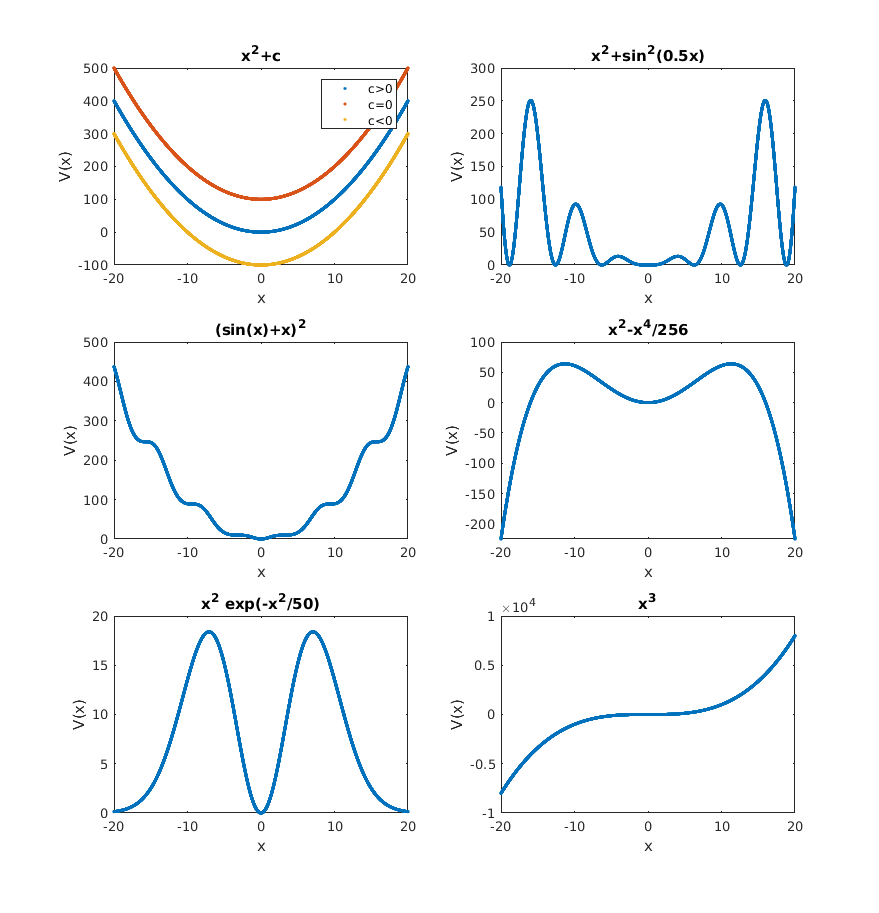
\includegraphics[scale=0.5, angle=0]{figs/fig_definite_functions.png}
  \caption{Illustration of definiteness properties of various functions.}
\end{figure}

Fig.\,(\ref{fig_definite_functions}) shows various functions which we will use to categorize definiteness.
\begin{enumerate}[noitemsep]
  \item Globally positive definite function; also radially unbounded as $V(x)\rightarrow\infty$ as $|x|\rightarrow \infty$. Note that in cases $a$ and $c$, we can shift coordinates to make them positive definite functions.
  \item Locally positive definite function over the open domain $(-2\pi,2\pi)$; also globally positive semi-definite.
  \item Globally positive definite function and radially unbounded.
  \item Locally positive definite function over the open domain $(-16,16)$; also locally positive semi-definite function over the closed domain $[-16,16]$.
  \item Globally positive definite function; however, not radially unbounded as $V(x)\rightarrow 0$ as $|x|\rightarrow\infty$.
  \item Indefinite function.
\end{enumerate}

\subsubsection*{Definiteness of a matrix}
We often have to deal with the definiteness of a matrix. The definiteness of matrix is defined based on the value of $\bm{x}^{\intercal}[\bm{K}]\bm{x}$ or the eigenvalues of the matrix.

$$
\bm{x}^{\intercal}[\bm{K}]\bm{x} = 
\begin{cases}
 >0&\implies\textnormal{ Positive definite (all positive eigenvalues)}\\  
 \geq0&\implies\textnormal{ Positive semi-definite (at least a zero other all positive eigenvalues)}\\  
 <0&\implies\textnormal{ Negative definite (all negative eigenvalues)}\\  
 \leq0&\implies\textnormal{ Negative semi-definite (at least a zero other all negative eigenvalues)}\\ 
 \textnormal{else}&\implies\textnormal{ Indefinite (combination of positive and negative eigenvalues)}
\end{cases}
$$

\subsection{Lyapunov functions}
Equipped with the idea of definiteness, we can not define Lyapunov functions. For a dynamical systems, proving a function to be Lyapunov function for that system allows us to prove stability. With all the definition, mathematics, and concepts we had to develop so far, this last step is very anti-climatic.

\textbf{Lyapunov function:} The scalar function $V(\bm{x})$ is a Lyapunov function for the dynamical system $\dot{\bm{x}}=\bm{f}(\bm{x})$ if it is continuous and there exists a $\delta>0$ such that for any $\bm{x}\in B_{\delta}(\bm{x}_{r})$
\begin{enumerate}[noitemsep]
  \item $V(\bm{x})$ is a positive definite function about $\bm{x}_{r}$
  \item $V(\bm{x})$ had continuous partial derivative
  \item $\dot{V}(\bm{x})$ is negative semi-definite.
\end{enumerate}

Particularly, Lyapunov function is a scalar function of those states of dynamical system that we want to control. It need not be function of all the states of the system. 

In the context of control theory, $V(\bm{x})$ is defined in terms to state variables \textit{relative to reference states}. When we write $V(\bm{x})$, (Lyapunov function as a function of $\bm{x}$) it implies that the reference is equilibrium point $\bm(x)_{r}=\bm{0}$. More generally, the Lyapunov function would be $V(\delta\bm{x})$ where $\delta\bm{x}=\bm{x}-\bm{x}_{r}$ is the error. We will encounter this in reference trajectory tracking problems. In this scenario, when the state error reaches the neighborhood $B_{\delta}(\delta\bm{x})$, we are constraining ourselves to be around that reference trajectory within the bound (Lyapunov stability) or converge (asymptotic stability).

Usually, we need to plug in the equation of motion of the dynamical system when we compute the derivative of the Lyapunov function. This is because while taking derivative using chain rule, we come across the term $\dot{\bm{x}}$ which is actually $\bm{f}(\bm{x})$.
$$
\dot{V}
=\frac{\partial V^{\intercal}}{\partial\bm{x}}\dot{\bm{x}} 
=\frac{\partial V^{\intercal}}{\partial\bm{x}}\bm{f}(\bm{x})\leq0
$$

\noindent
\textbf{Example:} Consider the spring-mass system
$$
m\ddot{x}+kx=0
$$

Let us use the total system energy as a candidate Lyapunov function.
$$
V(x,\dot{x}) = \frac{1}{2}m\dot{x}^{2}+\frac{1}{2}kx^{2}
$$

The Lyapunov rate is then expressed as
$$
\dot{V}(x,\dot{x}) = (m\ddot{x}+kx)\dot{x}=0\leq0
$$

Lyapunov functions are often inspired by energy, but they don't have to precisely be energy functions. Any functions that satisfies the properties can be a Lyapunov function. However,energy functions are good source of motivation to come up with mathematical structures that are quite convenient. For example, in the context of spring mass system, $V(x,\dot{x})$ is the sum of the kinetic energy and the spring potential energy. If we take the the derivative of $V(x,\dot{x})$, we will observe that it is always zero, hence satisfying the definition of the Lyapunov function. Since we can construct a Lyapunov function of spring-mass system for all states, the system is Lyapunov stable for all states. It should be noted that the Lyapunov function need not be valid for all possible states but a neighborhood.

\subsection{Lyapunov stability}
\textbf{Lyapunov stability:} If a Lyapunov function $V(\bm{x})$ exists for the dynamical system $\dot{\bm{x}} = \bm{f}(\bm{x})$., then the system is stable about the origin.

The requirement of $\dot{V}(\bm{x})$ to be negative semi-definite has a beautiful physical interpretation when in the context of Lyapunov stability. Negative semi-definite means that $\dot{V}(\bm{x})$ should either be negative or zero within the neighborhood. Suppose we consider energy function as the Lyapunov function of the system. This assumption suggests that the energy of the system will either decrease or stay constant. This intuition manifests itself directly in the definition of Lyapunov stability where the state should be within the bound; it need not converge and is allowed to oscillate within the bound. This allowance in oscillation within some bound (based on initial state) can be thought of the motion of dynamical system without loss in energy i.e. $\dot{V}(\bm{x})=0$. For example, if satellite tumbles and we bound it to desired magnitude by suitably choosing the initial condition, the rates will never increase. The worse it can get is continue tumble within the bound $(V(\bm{x}) = 0)$, but the rate might also decrease $(V(\bm{x})<0)$. 

However, if $\dot{V}(\bm{x})$ were to be negative definite, $V(\bm{x})$ had to be strictly decreasing i.e. asymptotic stable. 

\subsection{Asymptotic stability and LaSalle's invariance principle}
\subsubsection*{Asymptotic stability}
\textbf{Asymptotic Stability:} Assume $V(\bm{x})$ is a Lyapunov function about $\bm{x}_{r}(t)$ for the dynamical system $\dot{\bm{x}}=\bm{f}(\bm{x})$; then system is asymptotically stable if
\begin{enumerate}[noitemsep]
  \item the system is Lyapunov stable about $\bm{x}_{r}$, and
  \item $\dot{V}(\bm{x})$ is negative definite about $\bm{x}_{r}$.
\end{enumerate}

In this case, the states are forced to converge because $\dot{V}(\bm{x})$ is strictly negative. Oscillating within a bound forever is not allowed. However, it does not guarantee the performance. We cannot argue if it will converge slow or fast but all we know for sure is that it will converge.

\noindent
\textbf{Example}
Consider a spring-mass-damper system $$m\ddot{x}+c\dot{x}+kx=0$$ with Lyapunov function $$V(x,\dot{x})=\frac{1}{2}m\dot{x}^{2}+\frac{1}{2}kx^{2}$$.

Taking its derivative we get
$$
\dot{V}(x,\dot{x})=(m\ddot{x}+kx)\dot{x}=-c\dot{x}^{2}\leq0.
$$

Intuitively we know that damper forces the system to lose energy till it converge to equilibrium. However it is clearly not the case because $\dot{V}$ is only negative semi-definite. We see that the energy Lyapunov function fails to satisfy the asymptotic stability condition but shows Lyapunov stability. Actually there is some explanation hidden here. We know that negative semi-definiteness of the Lyapunov function suggests multiple local equilibria. However in case of this system, the states where $\dot{V}=0$ are transient states when the motion of mass is changing its direction (i.e. $\dot{x}=0$) i.e. when system is in motion. It is impossible fot the system to maintain $\dot{V}$ as an equilibrium without confining $\dot{x}$ to zero, which is possible if and only if $x\neq0$. This argument shows that even if $\dot{V}$ is negative semi-definite, it is impossible to maintain $\dot{V}$ unless it is origin. This argument clearly calls for extension of condition for asymptotic stability which is provided by LaSalle's invariance principle.

This example emphasizes an important feature of Lyapunov's stability theorem; namely, \textit{the theorem's conditions are only sufficient}. Failure of Lyapunov function candidate to satisfy the conditions fr stability (or asymptotic stability) does not mean that the equilibrium is not stable or asymptotically stable. It only means that such stability cannot be established by using this Lyapunov function candidate. Whether the equilibrium point is stable (asymptotically stable) or not can be determined only by further investigation. 

\subsubsection*{LaSalle's invariance principle}
Based on the argument we had in above section regarding the failure of Lyapunov function to establish the asymptotic stability, we can say formally, that if in a domain about the origin we can find a Lyapunov function whose derivative along the trajectories of the system is negative semi-definite, and if we can establish taht no trajectory can stay identically at points where $\dot{V}(x,\dot{x})=0$, except at origin, then the origin is asymptotically stable. This follows from LaSalle's invariance principle.

\textbf{Theorem} Assume there exists a Lyapunov function $V(\b{x}m)$ of the dynamical system $\dot{\bm{x}}=\bm{f}(\bm{x})$. Let $\Omega$ be the non empty set of state vectors such that
$$
\bm{x}\in\Omega\implies\dot{V}(\bm{x})=0
$$

If the first $k-1$ derivative of $V(\bm{x})$, evaluated on the set $\Omega$, are zero
$$
\frac{d^{i}V(\bm{x})}{dt^{i}}=0\quad\forall\bm{x}\in\Omega\quad i=1,2,3,...,k-1
$$

and the $k$-th derivative is negative definite on the set $\Omega$
$$
\frac{d^{k}V(\bm{x})}{dt^{k}}<0\quad\forall\bm{x}\in\Omega
$$

then the system $\bm{x}(t)$ is asymptotically stable if $k$ is an odd number.

The theorem says that if we take a set $\Omega$ of all the states where $\dot{V}(\bm{x})=0$. Now note that transient states and equilibrium states all comes under $\Omega$. What we need to do now is to filter out those transient states. Suppose you take $k-1$-th derivative of $V(\bm{x})$ and they are zeros, it means that till that point the system looks to be actually stuck in some equilibria because the energy function is not changing at all. But if we find that the $k$-th derivative is negative definite, this suggests that the $\dot{V}=0$ was instantneous case and it will eventually decrease leading us to equilibrium. Now the system is not in some equilibria but it is actually in motion and we got to consider it as transient condition. For mechanical systems, we typically have to look at second and third derivatives. Second derivative is usually sero and third negative definite leading the system to asymptotic stability.

\subsection{Projection of states to Lyapunov function}
\begin{figure}[ht]
  \label{fig_lyapunov_projection}
  \centering
  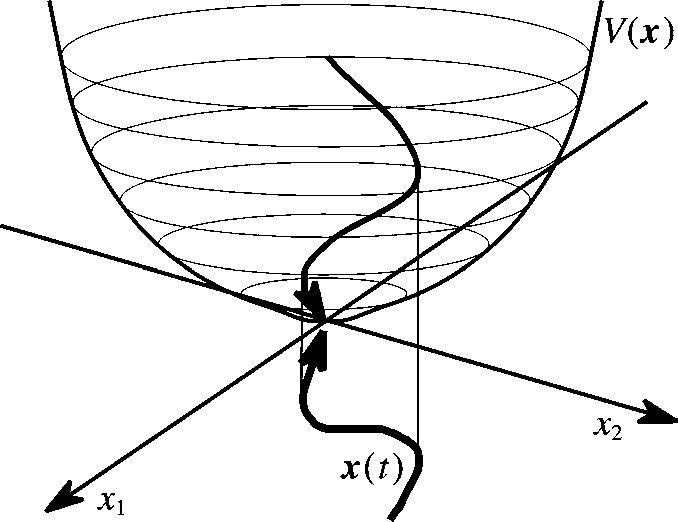
\includegraphics[scale=0.3, angle=0]{figs/fig_lyapunov_projection.png}
  \caption{Projection of motion of dynamical system on its Lyapunov function.}
\end{figure}

Fig\,(\ref{fig_lyapunov_projection}) shows that projection of the states of dynamical system on its Lyapunov function. It can be observed that the Lyapunov function restricts the scope of state of the system to keep it within the bound. Convergence is confirmed for asymptotic stability but not for Lyapunov stability. In case of Lyapunov stability, the state get closer to equilibrium of stay at same distance.

\subsection{Lyapunov stability of linear systems}
Using Lyapunov theory fo prove stability of linear system sounds overkill because we have all the beautiful tool of linear stability analysis. However sometimes a system might have linear and nonlinear part. In such cases Lyapunov stability analysis for linear system comes handy.

Let our dynamics be $\dot{\bm{x}}=[\bm{A}]\bm{x}$ where $[\bm{A}]$ is not time dependent (i.e. it is just a bunch of coeffifents). If we assume $[\bm{P}]$ be a symmetric positive definite matrix, now we can define Lyapunov function as

$$
V(\bm{x})=\bm{x}^{\intercal}[\bm{P}]\bm{x}.
$$

\begin{equation*}
\begin{split}
  \dot{V}&=\dot{\bm{x}}^{\intercal}[\bm{P}]\bm{x}+\bm{x}^{\intercal}[\bm{P}]\dot{\bm{x}}\\
         &=\bm{x}^{\intercal}([\bm{A}]^{\intercal}[\bm{P}]+[\bm{P}][\bm{A}])\bm{x}\\
\end{split}
\end{equation*}
To prove asymptotic stability, we need show that $[\bm{A}]^{\intercal}[\bm{P}]+[\bm{P}][\bm{A}]$ to be negative definite $[\bm{A}]^{\intercal}[\bm{P}]+[\bm{P}][\bm{A}]+[\bm{Q}]=0$ is also known as algebraic Lyapunov equation. There is a theorem that argues the definiteness of this term.

In this theorem $[\bm{A}],[\bm{P}],[\bm{Q}]\in\mathbb{R}^{n\times n}$. $[\bm{P}]$, and $[\bm{Q}]$ are symmetric.

\textbf{Theorem:} Given any $[\bm{Q}]>0$, there exists a unique $[\bm{P}]\succ0$ satisfying $[\bm{A}]^{\intercal}[\bm{P}]+[\bm{P}][\bm{A}]+[\bm{Q}]=0$ only if the linear system $\dot{\bm{x}}=[\bm{A}]\bm{x}$ is globally asymptotically stable. The quadratic function $V(\bm{x})=\bm{x}^\intercal[\bm{P}]\bm{x}$ is a Lyapunov function that can be used to verify stability.

The theorem suggests that the Linear dynamics is guaranteed to asymptotically converge it the algebraic Lyapunov equation exists for the system. In our formulation however, we do not have the matrix $[\bm{Q}\succ0]$, which suggests $[\bm{A}]^{\intercal}[\bm{P}]+[\bm{P}][\bm{A}]+[\bm{Q}]\prec0$ implies asymptotic stability. Without damping, we will have only marginal stability, this is handled by \textit{if and only if} in the theorem i.e $[\bm{A}]^{\intercal}[\bm{P}]+[\bm{P}][\bm{A}]+[\bm{Q}]\preceq0$ .

\subsection{Global stability}
The scope of the neighborhood within which the Lyapunov function is positive definite dictates if the stability (or asymptotic stability) is global or local. However, all the states satisfying the stability definitions is quite not enough for the system to be globally stable (or asymptotically stable). We also need to prove that the Lyapunov function is radially unbounded.

\textbf{Radially unbounded function} A function $f:\mathbb{R}^{n}\rightarrow\mathbb{R}$ is said to be \textit{radially unbounded function} if $$|\!|\bm{x}|\!|\rightarrow\infty\implies f(\bm{x})\rightarrow\infty.$$

Or equivalently,
$$\forall c>0:\exists r>0:\forall \bm{x}\in\mathbb{R}^{n}:[|\!|\bm{x}|\!|>r\implies f(\bm{x})>c]$$

Notice that the norm used in the definition can be any norm defined on $\mathbb{R}^{n}$, and the behavior of the function along the axes does not necessarily reveal that it is radially unbounded or not; i.e. to be radially unbounded, the condition must be verified along any path that results in $|\!|\bm{x}|\!|\rightarrow\infty$.

For example, the functions
\begin{equation*}
  \begin{split}
    f_{1}(\bm{x})&=(x_{1}-x_{2})^{2}\\
    f_{2}(\bm{x})&=\frac{x_{1}^{2}+x_{2}^{2}}{(1+x_{1}^{2}+x_{2}^{3})+(x_{1}-x_{2})^{2}}    
  \end{split}
\end{equation*}

are not radially unbounded since the axis along the line $x_{1}=x_{2}$, the condition is not verified even though the second function s globally positive definite.

We can also argue radially unboundedness by looking at the graph of the function. In first figure, $V(x)\rightarrow\infty$ as $x\rightarrow\infty$ so it is radially unbounded function. However in the second figure, $V(x)\rightarrow 0$ as $x\rightarrow\infty$, so the function is not radially unbounded so global stability cannot be argued for the second function.

In addition to Lyapunov function being positive definite for all possible states and its derivative negative semi-definite (or negative definite) it also should be radially unbounded to argue global stability (or asymptotic stability).

\section{Prototype Lyapunov Functions}
So far we are well equipped with the tools for nonlinear stability analysis; we know how to deal with stabilities once we are give a Lypaunov function for a dynamical system. However we still don't know how to originally come up with a Lyapunov function which is a challenging task. Energy is a big inspiration for Lyapunov functions and that is what we will start with. It should be noted that it is not always the case because we will use other mathematical structures (not energy functions) for CRP, MRPs and Quaternions. That being said, it is now time to make Lyapunov functions actually \textit{do something}.

We will break the analysis of Lyapunov function into rate and position based Lyapunov functions.

\subsection{General elemental rate Lyapunov function}
We will start our discussion with rates of general dynamical system; we are \textit{not} concerned about the positions itself.

\subsubsection{Regulation problem}
In the context of attitude control, we are interested in controlling the angular velocity of the spacecraft only and not orientation. In Gemini-8 mission two astronauts were trying to dock with another capsule. Something went wrong and they went tumbling. They were tumbling at crazy rates. It was amazing that they did not pass black out. They were able to figure out  that the wiring related to the firing strategy was mismatched. They were working on to improving it but ended up rotating at high angular rates. Finally they managed to stabilize. In this scenario, would the astronauts care about the final orientation of the spacecraft? No. They would want to stop the bloody rotation. That is the kind of control strategy we are going to talk about; Lyapunov control for tumbles (i.e. angular rates). We will not care about attitude but $\bm{w}$. In this particular context of Gemini mission, we want our angular rates to be at zeros which is a regulation problem.

We will work with form of general notation with which any mechanical systems can be written in. Working with dynamical system requires the familiarity with Lagrangian dynamics. The properties we are discussing in the form of general notation is powerful and we can apply it to wide ranges of mechanical systems and expand it to the particular system under study.

\begin{equation*}
  \begin{split}
  \textnormal{State vector }&:(\bm{q},\dot{\bm{q}})\\
  \textnormal{Goal}&:\dot{\bm{q}}\rightarrow0\\
  \textnormal{Kinetic energy}&:T=\frac{1}{2}\dot{\bm{q}}^{\intercal}[\bm{M}]\dot{\bm{q}}\quad\textnormal{where, }[\bm{M}]=[\bm{M}]^{\intercal}\succ0
  \end{split}
\end{equation*}

Kinetic energy becomes convenient positive definite measure for our errors (which are our rates when the goal are zeros). When we go through Lagrangian mechanics, we end with general equations:

$$
[\bm{M}(\bm{q})]\ddot{\bm{q}} = -[\dot{\bm{M}}(\bm{q},\dot{\bm{q}})]\dot{\bm{q}}+\frac{1}{2}\dot{\bm{q}}^{\intercal}[\bm{M}_{\bm{q}}(\bm{q})]\dot{\bm{q}}+\bm{Q}
$$

$\bm{Q}\in\mathbb{R}^{n}$ is generalized force vector which becomes control torque in attitude dynamics. $[\bm{M}\in\mathbb{R}^{n\times n}]$ is generalized mass matrix. For rotational dynamics (i.e. $[\bm{I}]\dot{\bm{w}}=-[\tilde{\bm{\omega}}][\bm{I}]\bm{\omega}+\bm{\tau}$), second term vanishes because the rate of change of inertial tensor relative to body frame is constant.

We need a Lyapunov function. The Lyapunov function need not be function of all the state variables of the dynamical system but it must be function of those parameters that we want to control. In our case, we are interested in the rates $\bm{\omega}$ so Lyapunov function must be the positive definite function of rates.

\begin{equation*}
  \begin{split}
    \textnormal{Lyapunov function}:V(\dot{\bm{q}})&=\frac{1}{2}\dot{\bm{q}}^{\intercal}[\bm{M}(\bm{q})]\dot{\bm{q}}\\
    \textnormal{Lyapunov rate}:\dot{V}&=\dot{\bm{q}}^{\intercal}[\bm{M}]\dot{\bm{q}}+\frac{1}{2}\dot{\bm{q}}^{\intercal}[\bm{M}]\dot{\bm{q}}\\
    &=\dot{\bm{q}}^{\intercal}\left(-\frac{1}{2}[\dot{\bm{M}}]\dot{q}+\frac{1}{2}\bm{q}^{\intercal}[\bm{M}_{\bm{q}}]\dot{\bm{q}}+\bm{Q}\right)\\
    &=\dot{\bm{q}}^{\intercal}\bm{Q}
  \end{split}
\end{equation*}

Here we are just waving hand and coming to the conclusion. Lots of fun mathematics goes into the derivation which is presented in the appendix \ref{section_generalized_lagrange_dynamics}. No matter how complex mechanical system is, whatever the generalized forces (mixtures of torques, and forces, and all the craziness) are, in the end it all boils down to this very simple form; the work energy principle. We will reexamine when we reach specific application where we can see how to incorporate motor torques and CMGs and so forth.

Now that we have $V$ and $\dot{V}$, we are looking for a control $\bm{Q}$ to arrest any $\dot{\bm{q}}$ and drive it to zero. We have freedom to pick forces and torques that acts on the system and there are infinitely may choices to be made. We are interested on the simple choice of $\bm{Q}$ which makes $\dot{V}$ negative definite as it would ensure asymptotic stability. Putting $\bm{Q}=-\dot{\bm{q}}$ does the job pretty nicely.
$$
\dot{V}=\dot{\bm{q}}^{\intercal}\bm{Q}=-\dot{\bm{q}}^{\intercal}\dot{\bm{q}}\prec0
$$

This is stable, actually asymptotically stable. What more, it is even globally asymptotically stable. This is really fantastic and The fact that we could prove global asymptotic stability on the complex nonlinear system and come up with a control law is the beauty of Lyapunov theory. But the question is; would you want to sit in the spacecraft with this control law? Maybe not. We have argued the stability but not performance. It is true that if we do not guarantee stability, forget performance its over but with stability we need to consider performance. How do we control the closed loop performance of this particular control law? There are no knob to tune and change the performance of control (maybe more aggressive or stiff). We can easily introduce this knob in the form of positive number.
$$
\bm{Q}=-k\dot{\bm{q}}^{\intercal}\dot{\bm{q}}\quad\quad\textnormal{where $k$ is positive gain}
$$

The beauty of this is that it does not change the stability argument because $\bm{Q}\prec0$ as long as the gain is positive. However it can change the performance. With the knob to tune, it behaves like a proportional feedback control which is linear. But the gain need not be a number, it can be a fully populated positive definite matrix. Instead of a single gain, now we have more complex system and multiple knobs to tune. Let $[\bm{P}]$ be a positive definite gain matrix.
$$
\dot{V}=-\dot{\bm{q}}^{\intercal}[\bm{P}]\dot{\bm{q}}\prec0\quad\quad\textnormal{(globally asymptotically stable)}
$$

Most often used gain matrix is in the form $[\bm{P}]=[\bm{I}]k$ where $k$ is a positive scalar and $[\bm{I}]$ is an identity matrix. It provides same gain across all axes.

\subsubsection{Tracking problem}
If your spacecraft is supposed to be scanning across the sky, it should have constant non-zero angular rates. In this situation you have the actual rate of the spacecraft, you compute error (i.e. deviation from expected rate), and try to match your rate to that non-zero value. This is a tracking problem. In tracking problems it is not the states that we want to drive to zero but the error so Lyapunov functions are often written in terms of errors.

Let us consider the tracking problem of a generalized mechanical system.
\begin{equation*}
  \begin{split}
  \textnormal{Reference states }&:(\bm{q}_{r},\dot{\bm{q}}_{r})\\
  \textnormal{State vector }&:(\bm{q},\dot{\bm{q}})\\
  \textnormal{Tracking error }&:\delta\bm{q}=\dot{\bm{q}}-\dot{\bm{q}}_{r}\\
  \textnormal{Goal}&:\delta\dot{\bm{q}}\rightarrow0\\
  \textnormal{Lyapunov function}&:V(\dot{\bm{q}})=\frac{1}{2}\delta\dot{\bm{q}}[\bm{M}(\bm{q})]\delta\dot{\bm{q}}\\
  \textnormal{Lyapunov rate}&:\dot{V}=\delta\dot{\bm{q}}^{\intercal}\left(-\frac{1}{2}[\dot{\bm{M}}](\dot{\bm{q}}+\dot{\bm{q}}_{r})+\frac{1}{2}\dot{\bm{q}}^{\intercal}[\bm{M}_{q}]\bm{\dot{q}}-[\bm{M}]\ddot{q}_{r}+\bm{Q}\right)\\
  \textnormal{Proposed control}&:\bm{Q}=\frac{1}{2}[\dot{\bm{M}}](\dot{\bm{q}}+\dot{\bm{q}}_{r})-\frac{1}{2}\dot{\bm{q}}^{\intercal}[\bm{M}_{q}]\dot{\bm{q}}+[\bm{M}]\ddot{q}_{r}-[\bm{P}]\delta\dot{\bm{q}}\\
  \textnormal{Lyapunov rate with control}&:\dot{V}(\delta\dot{\bm{q}})=-\delta\dot{\bm{q}}[\bm{P}]\delta\dot{\bm{q}}\prec0\quad\quad\textnormal{(globally asymptotically stabilizing)}
  \end{split}
\end{equation*}

We take natural step of using the energy-function-like positive definite measure of tracking error for Lyapunov function. This which has the energy-function like algebraic structure but is not exactly kinetic energy. We should note that the work/energy principle does not hold with these non-mechanical energy function, and ths Lyapunov rate is no longer the the simplified power equation.This function is positive definite because $[\bm{M}]$ is positive definite matrix. 

In computing $\dot{V}$, things just font drop out but we have all these terms with subscript $r$ on them. We can solve for $\bm{Q}$ and come up with and expression that will ensure $\dot{V}\prec0$ making the control law globally asymptotic stable. 

In regulation problem, we had proportional feedback part with the negative rate squared $(-\dot{\bm{q}}^{\intercal}[\bm{P}]\dot{\bm{p}})$ and all was good but it is quite elaborate in tracking problem where we have feedforward reference motion terms (terms with subscript $r$). Since we are trying to catchup with $\dot{\bm{q}}_{r}$ we will start by imposing torque for ideal nominal angular rates that the spacecraft should have. This feedforward compensation with the feedback control effort makes the complete control law. It should be noted that the reference is allowed to be time varying as well, in such cases we might have to accelerate, slow down, and accelerate again based on the angular rate trajectory.

\subsection{Applications of general elemental rate Lyapunov function}
The regulation and tracking problem that we did for angular rates are applied to generalized system. We will see an example of a multi-link system before applying to the rotational dynamics of rigid body.

\subsubsection{Multi-link system rate control}
\begin{equation*}
  \begin{split}
    \textnormal{State vector }&:\bm{q}=[\theta_{1},\theta_{2},\theta_{3}]^{\intercal}\\
    \textnormal{Goal}&:\delta\dot{\bm{q}}\rightarrow0\\
    \textnormal{Equations of motion}&:[\bm{M}]\ddot{\bm{q}}+[\dot{\bm{M}}]\dot{\bm{q}}-\frac{1}{2}\dot{\bm{q}}^{\intercal}[\bm{M}(\bm{q})]\dot{\bm{q}}\\
    \textnormal{Lyapunov function}&:\bm{V}(\dot{\bm{q}})=\frac{1}{2}\dot{\bm{q}}^{\intercal}[\bm{M}(\bm{q})]\dot{\bm{q}}\\
    \textnormal{Lyapunov rate}&:\dot{V}=\dot{\bm{q}}^{\intercal}\bm{Q}\\
    \textnormal{Controls}&:\bm{Q}_{1}=-[\bm{P}_{1}]\dot{q}\quad\quad\quad\quad\textnormal{(Rate feedback)}\\
    &:\bm{Q}_{2}=-[\bm{P}_{2}][\bm{M}(\bm{q})]\dot{q}\quad\textnormal{(Momentum feedback)}\\
  \end{split}
\end{equation*}

Where $[\bm{M}(\bm{q})]$ is positive definite and symmetric mass matrix.
$$
[\bm{M}(\bm{q})]=
\begin{bmatrix}
  (m_{1}+m_{2}+m_{3})l^{2}_{1} & (m_{2}+m_{3})l_{1}l_{2}\cos{(\theta_{2}-\theta_{1})} & m_{3}l_{1}l_{3}\cos{(\theta_{3}-\theta_{2})}\\
  (m_{2}+m_{3})l_{1}l_{2}\cos{(\theta_{2}-\theta_{1})} & (m_{2}+m_{3})l^{2}_{2} & m_{3}l_{1}l_{3}\cos{(\theta_{3}-\theta_{2})}\\
  m_{3}l_{1}l_{3}\cos{(\theta_{3}-\theta_{2})} & m_{3}l_{1}l_{3}\cos{(\theta_{3}-\theta_{2})} & m_{3}l^{2}_{3}
\end{bmatrix}
$$

Here is a general mechanical system which is not a rigid body but a multi-link system with three links. It could be an approximation of a flexible system or a multi-hinged deployable solar panels. We can observe that $[\bm{M}]$ depends on the configurations of multi-link system. Suppose this system is thrown out and is jiggling and wiggling and gyrating. Our goal is to make it come to rest without worrying about the angles of each link.

We will take a look at two different control laws, both of whom end up making $\dot{V}$ negative definite. Hence we have globally asymptotically stabilizing control law but this is beginning of control development. Next important thing that we need to consider is the performance of these controls. In the simulation result with $\bm{Q}_{1}$ we see that initially one of the links have rate but remaining two are at rest. If we let the system evolve with $\bm{Q}_{1}$ control, motion of the first link pulls on the second one and so on. All three links start moving. In this control we are sacrificing; we are getting rid of te kinetic energy of the third link by adding some kinetic energy in the first two. With this dissipative effect, we are guaranteed to stabilize asymptotically.

The application of control $\bm{Q}_{2}$ with its angular momentum feedback produces different behavior. The first two links barely budge as the third link is brought to rest. This is because this control immediately applies control to third link to slow it down but that the same time providing torques to other two links to keep them steady. This is the feature which the first controller was incapable of. The point is that there are whole variety of control laws that we can come with that are stable but we need to go for the one that has good performance.

\subsubsection{Rigid body detumble}
\begin{equation*}
  \begin{split}
    \textnormal{State vector }&:\bm{\omega}\\
    \textnormal{Goal }&:\bm{\omega}\rightarrow0\\
    \textnormal{Equations of motion }&:[\bm{I}]\dot{\bm{\omega}}=-[\tilde{\bm{\omega}}][\bm{I}]\bm{w}+\bm{Q}\\
    \textnormal{Lyapunov function }&:V(\dot{\bm{\omega}})=T=\frac{1}{2}\bm{\omega}^{\intercal}[\bm{I}]\bm{\omega}\\
    \textnormal{Lyapunov rate }&:\dot{V}=\bm{\omega}^{\intercal}([\bm{I}]\dot{\bm{\omega}})\\
    &=\bm{\omega}^{\intercal}(-[\tilde{\bm{\omega}}][\bm{I}]\bm{\omega}+\bm{Q})\\
    &=\bm{\omega}^{\intercal}\bm{Q}\\
    \textnormal{Control }&: \bm{Q}=-[\bm{P}]\bm{\omega}\quad\quad[\bm{P}]=[\bm{P}]^{\intercal}\succ0\\
    \textnormal{Lyapunov rate with control}&:\dot{V}(\dot{\omega})=-\bm{\omega}^{\intercal}[\bm{P}]\bm{\omega}\succ0\\
  \end{split}
\end{equation*}

In this dynamical system we only care about the rate $\bm{\omega}$. The kinetics differential equation has a control $\bm{Q}$ which allows us to do so. We have not considered any perturbations so $\bm{Q}$, in this case, does not represent any external torques. Our goal is to drive $\bm{\omega}$ to zero which is a regulation problem. The kinetic energy is used as candidate Lyapunov function which is expressed in terms of states we care about (i.e. rates). $[\bm{I}]\succ0$ so all is good. 

We know that the Lyapunov function is a scalar hence there is no time dependency. However, on the right hand side, there are bunch of vectors and tensors which are frame dependent. So with respect to which frame should we take the derivative? Body frame. It is because inertial tensor remains constant in body frame and it makes life easier.

The process is pretty mush similar with general element rate control with which arrive at the control law which guarantee the Lyapunov rate to be positive definite. $[\bm{P}]$ is control gain matrix which controls the performance if you want to make your detumbling sluggish or stiff. The final $\dot{V}$ is negative definite and radially unbounded as well so the system is globally asymptotically stable. 

Let us examine what our control law is dependent on. What are the feedback that the control $\bm{Q}$ require? Angular rates $(\bm{\omega})$. No attitude. No inertia tensor. Actually the study of Lyapunov optimal and saturated controls will show that we \textit{don't even have to know} rates perfectly as long as we get the sign right. So if the angular velocity if $0.2$ rad/s or $-0.2$rad/s, all we are interested is the sign and still the control will be stable.

Let us see why independence to inertial tensor is important. Let us imagine a robotic docking system trying to grab boulders, we do not know exactly what that mass is going to be. Robot picks up a heavy boulder and tends to tumble because with the added mass to the system, the inertial tensor is now different and the control gains might not work for this \textit{new system}. In such cases if we have a control law that does not depends on the inertia tensor then it will prove to be very robust. Ensuring global stability with no infinite insensitivity to inertia tensor or mass properties is really fantastic.

\subsubsection{Rigid body rate tracking}
\begin{equation*}
  \begin{split}
    \textnormal{Reference }&:\bm{\omega}_{r}\\
    \textnormal{Goal }&:\delta\bm{\omega}-\bm{\omega}_{r}\rightarrow0\\
    \textnormal{Note}&:{}^{B}\delta\bm{\omega}={}^{B}\bm{\omega}-[BR]{}^{R}\bm{\omega}_{r}\\
    \textnormal{Lyapunov function}&:V(\delta\bm{\omega})=\frac{1}{2}\delta\bm{\omega}^{\intercal}[\bm{I}]\delta\bm{\omega}\\
    \textnormal{Lyapunov rate}&:\dot{V}=\delta\bm{\omega}^{\intercal}[\bm{I}]\frac{{}^{B}d}{dt}(\delta\bm{\omega})\\
    &=\delta\bm{\omega}^{\intercal}(-[\tilde{\bm{\omega}}][\bm{I}]\bm{\omega}+[\bm{I}]\bm{\omega}\times\bm{\omega}_{r}-[\bm{I}]\dot{\bm{\omega}}_{r}-[\bm{I}]\dot{\bm{\omega}}_{r}+\bm{Q})\\
    \textnormal{Note}&:\frac{{}^{B}d}{dt}(\delta\bm{\omega})=\dot{\bm{\omega}}-\dot{\omega}_{r}+\bm{\omega}\times\bm{\omega}_{r}\\
    \textnormal{Control}&:\bm{Q}[\tilde{\bm{\omega}}][\bm{I}]\bm{\omega}+[\bm{I}][\tilde{\bm{\omega}}]\bm{\omega}_{r}+[\bm{I}]\dot{\bm{\omega}}_{r}-[\bm{P}]\delta\bm{\omega}\\
    \textnormal{Lyapunov rate with control}&:\dot{V}(\delta\bm{\omega})=-\delta\bm{\omega}^{\intercal}[\bm{P}]\delta\bm{\omega}\prec0\\
  \end{split}
\end{equation*}

In tracking problem there is a reference $\bm{\omega}_{r}$ that we want to follow. This means we want our spacecraft to spin about particular axes so that particular scan mission is achieved. The reference could be time varying as well. The state that we care about is $\delta\bm{\omega}$. When we write the Lyapunov function, our ${}^{B}\delta\bm{\omega}$ (i.e. rates of $B$ relative to $N$) equals ${}^{B}\bm{\omega}-[BR]{}^{R}\bm{\omega}_{r}$. We must make sure everything are written in same frame while doing computations. For control, there is never just one Lyapunov function to prove stability, We have factor of $\frac{1}{2}$ which drops due to differentiation. It is good because we don't want the factor floating around and anyways the stability argument is not violated. When it comes to differentiation, we like body frame derivatives because $[dot{\bm{I}}]=0$ in body frame. The body frame derivative ${}^{B}\bm{\omega}_{N}$ is performed with respect to the inertial frame which is not same as ${}^{B}\bm{\omega}_{R}$ which is performed relative to the reference frame. That is why we do transport theorem.

Arriving to control which makes $\dot{V}$ is pretty easy; we solve for $\bm{Q}$ by setting $\dot{V}=-\delta\bm{\omega}^{\intercal}[\bm{P}]\delta\bm{w}$. We observe that this control requires $\bm{I}$ so it is necessary to study the sensitivity of control for change in $\bm{I}$. What is inertia if off by $5\%$? It turns out that it is quire robust. You can be off by many 10s of percent and it will still work reasonably well. But the performance will be different. It depends upon knowledge ot inertia. You have to feedforward the reference acceleration of angular velocity. Keep in mind that there are no coordinate framed defined hare. The $\bm{\omega}_{r}$ is typically given in reference frame components. Your $\bm{\omega}$ is typically ${}^{B}\bm{\omega}$ which is measured in body frame components. So these equations are written in a frame agnostic way. During the implementation, we need to make sure that everything are in same frame. We cannot perform basic operations like addition if the vectors are not in same reference frame. Make sure rates in in $R$ frame ${}^{R}\bm{\omega}$ gets mapped to rates in $B$ frame ${}^{B}\bm{\omega}$ i.e. everything has to be in body frame. The fact that every vectors are in same frame will be implied in out discussions.

Lets examine the control law and discuss its saturation. The control depends quadratically on $\bm{\omega}$ i.e. $([\tilde{\bm{\omega}}][\bm{I}]\bm{\omega}_{r}$). So if you have really fast tip-off rates, fast squared gets really really fast and if your control depends on it, we might not have enough control to come up to that value. This case is known as saturation where the stability assumes unlimited control authority by actuators which we cannot provide. This can be a issue, however we can do a trick with rate functions to get rid of this problem.

To derive $\bm{Q}$, we took the system, selected a candidate Lyapunov function, derived $\dot{V}$, set $\dot{V}=-\delta\bm{\omega}^{\intercal}[\bm{P}]\delta\bm{w}$, and solved for $\bm{Q}$. There is another path we could follow. Instead of having $[\tilde{\bm{\omega}}][\bm{I}]\bm{\omega}$, we can put a control that says $[\tilde{\bm{\omega}}_{r}][\bm{I}]\bm{\omega}$. We are making some subtle changes to control. It will not cancel the term $[\tilde{\bm{\omega}}_{r}][\bm{I}]\bm{\omega}$ in $\dot{V}$ but something more interesting.

\begin{equation*}
  \begin{split}
    &-[\tilde{\bm{\omega}}][\bm{I}]\bm{\omega}+[\tilde{\bm{\omega}}_{r}][\bm{I}]\bm{\omega}\\
    =&-[\tilde{\bm{\omega}-\bm{\omega}_{r}}][\bm{I}]\bm{\omega}\\
    =&-\delta\tilde{\bm{\omega}}[\bm{I}]\bm{\omega}\\
  \end{split}
\end{equation*}

If we look at $\dot{V}$, everything is multiplied with $\delta\bm{\omega}$. $\delta\tilde{\bm{\omega}}$ dotted or transposed with something $(\delta\bm{\omega})^{\intercal}$ is a wonderful identity for $\delta\bm{\omega}^{\intercal}\delta\bm{\omega}$. We can guarantee both of the controls to be asymptotically stable and one of them depends linearly with the rates while the other one depends quadratically. The better between these two is judge based on their respective performance comparison. If you have high control authority, quadratic part might give you better closed loop performance.  Stability and performance are arguments of different level because we saw in multi-link system on how important performance criteria can be. However performance does not have absolute notion; a controller rejected by one might be useful to other on different aspect. 

\subsection{General elemental state Lyapunov function}
It is time to look at position based functions (not the rates) where we will be searching positive definite functions in terms of position coordinates. Easy measure is always to think upfront like spring energy which means that if there is some value you are not where you should be. If it decays then you are back where you should be. If you think of spring mass damper like things, we can use positive definite function like potential energy $(0.5kx^{2})$. We can do this for Euler angles and for different parameterizations. We will discuss pluses and minuses of each. Now we only care about control of attitude only and from the control prospective, $\bm{\omega}$ is our control variable.

We can also do attitude \textit{and} rate control simultaneously in which case things couple fully and $\bm{\omega}$ sample out but for now, let us start with only attitude.

\subsection{Applications of general elemental state Lyapunov function}
\subsubsection{Euler angles}

\paragraph{Regulation problem}
\begin{equation*}
  \begin{split}
    \textnormal{State vector}&:\bm{\theta}=[\theta_{1},\theta_{2},\theta_{3}]^{\intercal}\\
    \textnormal{Lyapunov function}&:V(\bm{\theta})=\frac{1}{2}\bm{\theta}^{\intercal}[\bm{K}]\theta\quad\quad[\bm{K}]=[\bm{K}]^{\intercal}\succ0\\
    \textnormal{Kinematics}&:\dot{\bm{\theta}}=[\bm{B}(\bm{\theta})]\bm{\omega}\\
    \textnormal{Lyapunov rate}&:\dot{V}=\bm{\omega}^{\intercal}([\bm{B}(\bm{\theta})]^{\intercal}[\bm{K}]\bm{\theta})\\
  \end{split}
\end{equation*}

Let $\bm{\theta}=[\theta_{1},\theta_{2},\theta_{3}]^{\intercal}$ be our Euler angles. The steps are basically the one we have already done in previous examples; take derivative of Lyapunov function, plug in the dynamics and so on. We have to notice that the Lyapunov function is in the form of spring-energy. However, it was in the form of kinetic energy when dealing with rates. So we basically have our building lego blocks. If we want to rates we use the kinetic energy whereas if we use the attitude, we use this quadratic measure. Remember the rotation matrix $[\bm{B}]$ has singularities. There are certain attitudes, pitch and steer inclinations that gives us issues which immediately makes $\dot{V}$ a nonlinear function; your control should be nonlinear which have to deal with such singularities. So Euler angles for general tumbling is not a good choice.

\paragraph{Tracking problem}
\begin{equation*}
  \begin{split}
    \textnormal{Attitude error (of $B$ wrt. $R$))}&:\bm{\theta}=[\theta_{1},\theta_{2},\theta_{3}]^{\intercal}\\
    \textnormal{Kinematics}&:\dot{\bm{\theta}}=[\bm{B}(\bm{\theta})]\delta\bm{\omega}\quad\quad\delta\bm{\omega}=\bm{\omega}-\bm{\omega}_{r}\\
    \textnormal{Lyapunov function}&:V(\bm{\theta})=\frac{1}{2}\bm{\theta}^{\intercal}[\bm{K}]\theta\\
  \end{split}
\end{equation*}

For tracking problems, Euler angles of body frames are defined relative to the reference frame. Values of Euler angles basically mean from the reference, what 321 sequence do you have to do so that you get to attitude of the body frame. This attitude of body frame relative to reference is our error attitude so $\delta\bm{\theta}$ and $\delta\bm{\omega}$ that we are dealing with are attitude and rates of body frame relative to reference frame. Usually we express the states in reference frame when we deal with tracking problems. We can see that Lyapunov functions in both cases are pretty similar that is why we will not consider both regulation and tracking problems for other parameters as math is pretty identical. The only and important difference is that we are talking about the attitude relative to different coordinate axes.

\subsubsection{Classical Rodrigues Parameters}
$$
V(\bm{q})=\bm{q}^{\intercal}[\bm{K}]\bm{q}
$$
Taking the derivative we get
$$
\dot{V}=\bm{\omega}^{\intercal}((\bm{I}-[\tilde{\bm{q}}]+\bm{q}\bm{q}^{\intercal})[\bm{K}]\bm{q})
$$
which gets reduced to 
$$
\dot{V}=\bm{\omega}^{\intercal}(K(1-q^{2})\bm{q})
$$
if the gain matrix $[\bm{K}]$ is replaced by a scalar $K$ and $q^{2}=\bm{q}\bm{q}^{\intercal}$.

The quadratic term $q^{2}$ may lead to nonlinear feedback laws. There is a more elegant Gibbs-vector Lyapunov function which is given by
$$
V(\bm{q})=K\ln((1+\bm{q}^{\intercal}\bm{q}))
$$

Taking the derivative, and substituting the differential kinematic equations, a surprisingly simple form is found.
$$
\dot{V}=\bm{\omega}^{\intercal}(K\bm{q})
$$

This leads to linear attitude feedback control. Let us develop a servo law, we define
$$
V(\bm{q})=\ln{(1+\bm{q}\bm{q}^{\intercal})}\textnormal{ with }\dot{V}=\bm{\omega}.
$$

The body rate control vector is then defined as
$$
\bm{\omega}=-[\bm{K}]\bm{q}\implies\dot{V}(\bm{q})=-\bm{q}^{\intercal}[\bm{K}]\bm{q}\prec0
$$

CRPs are nice because you can go from having singularity being no more than $90^{\circ}$ away (Euler angles) to having singularity being $180^{\circ}$ away from your reference. This is nice but still we cannot yet do complete tumbling without singularity. We can use the quadratic measure as Lyapunov function by eliminating the factor $1/2$ because differential kinematic equation for CRP already has the factor and we don't want to end up with bunch of 2s or 1/2s/
 
A brute force approach would define a candidate Lyapunov function as spring-mass energy-like form which is convenient and when we plug in $\dot{\bm{q}}$, we can see that $q^{2}$ makes $\dot{V}$ a nonlinear equation. It is simple and does not have crazy zeros or zero singularities. However at $180^{\circ}$, it $\bm{q}$ will blow up.

Panagiotis Tsiotras came up with wonderful approach of using natural log functions as Lyapunov functions which is very elegant. We take the Lyapunov function, take the log derivative and lo and behold; we end up with $\dot{V}=\bm{\omega}^{\intercal}(K\bm{q})$. This $\dot{V}$ is very amazingly simple and beautiful. However, it does not allow positive definite gain matrix to be with $\bm{q}^{\intercal}\bm{q}$ a scalar outside or none of this magic mathematics will work. So to use this function, you need to have equal gain along all axes of attitude error. If tou need more freedom with the gain, you might have to come up with a Lyapunov function and prove the stability of system with the function. The second Lyapunov function led to linear attitude control which shows that we can prove global stability without necessarily having nonlinear control for nonlinear dynamics.

Note how we are treating angular velocity (instead of torque) as our control variable. Now need to make servo controls to make sure that the spacecraft catchup with the angular rate commands calculated by the control laws we designed. In robotics, they don't do controls like the way we are doing. There are very complex mechanical systems and they try to do everything in the control torque level which is very challenging. When, instead, we are using UAV or robots, we give commands using joystick for forward and back and forth. Every time you give command, it is a speed. Now there is servo control implemented in the robot which catchups with the rate you command using joystick. So, in these cases, there are servo subsystems that tracks the commanded rates. We can do basically same with spacecrafts. The control $\bm{\omega}$ commands generated using Lyapunov method becomes reference rates to this servo subsystem which takes feedback from gyro sensor and drive the rate of spacecraft to the reference. All we need to do is to make sure that the reference $\bm{\omega}$ are generated with a control law that guarantees the global stability.

\subsubsection{Modified Rodrigues Parameters}

\begin{equation*}
  \begin{split}
    \textnormal{Lyapunov function}&:V(\bm{\sigma})=2K\ln{(1+\bm{\sigma}^{\intercal}\bm{\sigma})}\\
    \textnormal{Lyapunov rate}&:\dot{V}=\bm{\omega}^{\intercal}(K\bm{\sigma})\\
  \end{split}
\end{equation*}

If you switch to the shadow MRP sth on the $\sigma^{2}=1$ surface, then this Lyapunov function is continuous.

This leads to elegant linear attitude feedback laws which are globally stabilizing by switching between the original and shadow MRP set.

MRPs have similar properties as that of CRPs. Notice that there is a factor two in $V$ which is because there is 1/4 in the kinematics of MRP. Tsiotras came up with the idea that with $1+\bm{\sigma}\bm{\sigma}$ measure, we can get linear dependence of $V$ on $\bm{\sigma}$ leading to linear control which is also globally asymptotically stable without singularities. While using MRPs, we technically switch at $\sigma^{2}=1$ at which the attitude of body frame relative to reference is $180^{\circ}$. This means that getting upside down is the worst possible state you can be in; if more than $180^{\circ}$, it gets better again. If we look at the Lyapunov function, even with the switchingm $V$ is continuous but not necessarily continuously differentiable. With switching, we need to make extra arguments to prove stability for which we look at switched Lyapunov structures. But continuity is the key aspect, and it is satisfied with this Lyapunov function in terms of MPRs. We wil switch when we are upside down but continuity is not violated.

Note that we will stabilize the attitude to $\beta_{0}=\pm1$, which is the same attitude. However, no guarantee is made if the long or short rotational path is used.

\subsubsection{Quaternions}
\begin{equation*}
  \begin{split}
    \textnormal{Ideal attitude}&:\hat{\bm{\beta}}=[1,0,0,0]^{\intercal}\\
    \textnormal{Lyapunov function}&:V(\bm{\beta})=K(\bm{\beta}-\hat{\bm{\beta}})^{\intercal}(\bm{\beta}-\hat{\bm{\beta}})\\
    \textnormal{Lyapunov rate}&:\bm{V}=K\bm{\omega}^{\intercal}[\bm{B}({\bm{\beta}})]^{\intercal}(\bm{\beta}-\hat{\bm{\beta}})\textnormal{ where }[\bm{B}({\bm{\beta}})]^{\intercal}\bm{\beta}=0\\
    &= K\bm{\omega}^{\intercal}[\beta_{1},\beta_{2},\beta_{3}]^{\intercal}=\bm{\omega}^{\intercal}(K\epsilon)
  \end{split}
\end{equation*}

When using quaternions, often the reference attitude is set to zero rotation quaternion. We should note that quaternion with all zero violates the unit norm constraint so whenever we say zero quaternion, we mean the quaternion which represents zero rotation and aligns the body frame to the reference frame i.e. $[1,0,0,0]^{\intercal}$. When we drive the quaternion relative to reference to zero, it means that the error of orientation of body frame relative to reference is being driven to zero. So the ultimate control goal is $beta_{0}=1$ and $\beta_{1}=\beta_{2}=\beta_{3}=0$. We can derive things following the process we established before. There is a problem however, $\beta_{0}\pm1$ represents same orientation ($360^\circ$ rotation). If you perform control to $\beta_{0}=-1$, you are basically commanding the spacecraft to make $359^{\circ}$ rotation to correct for error of $1^{\circ}$. Any more, it goes back to $+1$ and we never track more than 1 revolution with quaternion with this control which is a \textit{windup problem}. So, we should manually handle this peculiarity in software which the control does not do for us. So with this control law, you are sure to achieve the stability to drive your error quaternion to zero but there is a possibility of the spacecraft taking long route of rotation. This can be eliminated by handling the signs of error quaternion.

We see that with MRP and quaternions, we came up with simple linear control law to stabilize nonlinear attitude dynamics. However in implementation, we must to handle switching for both of them to avoid singularities and windup for MRPs and quaternions respectively.

\subsection{Review}
\begin{enumerate}
  \item Kinetic energy is good Lyapunov candidate function for only rate control.
  \item Spring-energy like functions are good candidate function for only position control.
  \item In CRP we introduced the use of natural logarithm as Lyapunov function.
  \item In regulation problems, we are expressing our attitude and rates of body frame with respect to the inertial reference frame.
  \item In tracking problems, we express our attitude and rates of body frame with respect to the reference frame which we are trying to track.
  \item In the attitude control problems, angular rates are chosen as control variable. A servo subsystem is implemented for spacecraft to track these rates.
\end{enumerate}

\section{Attitude Control of States and Rates}
We worked out Lyapunov analysis for separate cases of rate control and state control and are provided with building blocks which we can put together to construct control for both rate \textit{and} state variables. Regulation problem is special case of the tracking problem which is mathematically elaborate, so we will start with tracking problem. Our goal is to look for a control law that is asymptotically stable for both rates and states.

\subsection{Tracking problem}
\begin{equation*}
  \boxed{
  \begin{split}
    \textnormal{Kinetics}&:[\bm{I}]\dot{\bm{\omega}}=-[\tilde{\bm{\omega}}][\bm{I}]\bm{\omega}+\bm{u}+\bm{L}\\
    \textnormal{Kinematics}&:\dot{\sigma} = \frac{1}{4}\left[(1-\sigma^{2})[\bm{I}]+2[\tilde{\bm{\sigma}}]+2\bm{\sigma}\bm{\sigma}^{\intercal}\right]\delta\bm{\omega}\\
    \textnormal{Error rate}&:\delta\bm{\omega}=\bm{\omega}_{\mathcal{B}/\mathcal{R}}=\bm{\omega}-\bm{\omega}_{r}\\
    \textnormal{Error attitude}&:\bm{\sigma}=\bm{\sigma}_{\mathcal{B}/\mathcal{R}}\\
    \textnormal{Lyapunov function}&:V(\delta{\bm{\omega}},\bm{\sigma})=\frac{1}{2}\delta\bm{\omega}^{\intercal}[\bm{I}]\delta\bm{\omega}+2k\ln(1+\bm{\sigma}^{\intercal}\bm{\sigma})\\
    \textnormal{Lyapunov rate}&:\dot{V}=\delta\bm{\omega}^{\intercal}\left([\bm{I}]\frac{{}^{\mathcal{B}}d}{dt}(\delta\bm{\omega})+K\bm{\sigma}\right)=\delta\bm{\omega}^{\intercal}[\bm{P}]\delta\bm{\omega}\\
    \textnormal{Control law}&:\bm{u}=-K\bm{\sigma}-[\bm{P}]\delta\bm{\omega}+[\bm{I}](\dot{\omega}_{r}-[[\tilde{\bm{\omega}}]\bm{\omega}_{r}])+[\tilde{\bm{\omega}}][\bm{I}]\bm{\omega}-\bm{L}\\
  \end{split}
  }
\end{equation*}

The Lyapunov candidate function for both attitude and rate control are the sum of Lyapunov function that we used to individually attitude and rate control. This is where the idea of building blocks in the context of Lyapunov analysis comes into play i.e. you can use the sum of individual Lyapunov functions for different states for argument analysis of union of those states.

\begin{equation}
  \label{eqn_rate_attitude_lyapunov}
  V(\delta{\bm{\omega}},\bm{\sigma})=\frac{1}{2}\delta\bm{\omega}^{\intercal}[\bm{I}]\delta\bm{\omega}+2k\ln(1+\bm{\sigma}^{\intercal}\bm{\sigma})
\end{equation}

Let us explore the properties of this Lyapunov function.

\begin{enumerate}
  \item $V(\delta\bm{\omega},\bm{\sigma})\succ0$
  \item $V(\delta\bm{\omega},\bm{\sigma})\rightarrow\infty\implies\text{ either }\delta{\bm{\omega}}\rightarrow\infty\text{ or }\bm{\sigma}\rightarrow\infty$
\end{enumerate}

Radially unbounded positive definiteness of $V(\delta\bm{\omega},\bm{\sigma})$ suggests that we are in right track for designing asymptotically stable control on $\delta\bm{\omega}$ and $\bm{\sigma}$. However, analysis of $\dot{V}$ is yet to be done before arguing the stability. Computing $\dot{V}$ gives us,

\begin{equation*}
  \dot{V}=\delta\bm{\omega}^{\intercal}\left([\bm{I}]\frac{{}^{\mathcal{B}}d}{dt}(\delta\bm{\omega})+K\bm{\sigma}\right)
\end{equation*}

Let us force the term in bracket to be $-[\bm{P}]\delta\bm{\omega}$. Which gives the closed loop dynamics of $\delta\bm{\omega}$.

\begin{equation}
  \label{eqn_error_rate_cld}
  [\bm{I}]\frac{{}^{\mathcal{B}}d}{dt}(\delta\bm{\omega})+[\bm{P}]\delta\bm{\omega}+K\bm{\sigma}=0  
\end{equation}

Here is a problem. Above substitution makes $\dot{V}=\delta{\bm{\omega}}^{\intercal}[\bm{P}]\delta\bm{\omega}$ which is only positive definite to $\delta\bm{\omega}$ but not $\bm{\sigma}$. With this $\dot{V}$, we cannot argue asymptotic stability of attitude $\bm{\sigma}$ using Lyapunov analysis (but that does not mean it is not asymptotically stable). However, if we come up with control that leads to above closed loop dynamics of $\delta\bm{\omega}$, we can prove the system to be globally stable (not convergence). Let us proceed with it.

The body frame derivative of the $\delta\bm{\omega}$ can be computed using transport theorem.

\begin{equation}
  \label{eqn_transport_theorm}
  \frac{{}^{\mathcal{B}}d}{dt}(\delta\bm{\omega})=\dot{\bm{\omega}}-\dot{\bm{\omega}}_{r}+\bm{\omega}\times\bm{\omega}_{r}
\end{equation}

Substituting Eqn.(\ref{eqn_transport_theorm}) on Eqn.(\ref{eqn_error_rate_cld}), we can compute the control that satisfied the closed loop response Eqn.(\ref{eqn_error_rate_cld}).

\begin{equation}
  \label{eqn_rate_attitude_tracking}
  \begin{split}
    &[\bm{I}](\dot{\bm{\omega}}-\dot{\bm{\omega}}_{r}+\bm{\omega}\times\bm{\omega}_{r} )+[\bm{P}]\delta\bm{\omega}+K\bm{\sigma}=0\\
    \text{or, }&[\bm{I}]\dot{\bm{\omega}}-[\bm{I}]\dot{\bm{\omega}}_{r}+[\bm{I}][\tilde{\bm{\omega}}]\bm{\omega}_{r}+[\bm{P}]\delta\bm{\omega}+K\bm{\sigma}=0\\
    \text{or, }&-[\tilde{\bm{\omega}}][\bm{I}]\bm{\omega}+\bm{u}+\bm{L}-[\bm{I}]\dot{\bm{\omega}}_{r}+[\bm{I}][\tilde{\bm{\omega}}]\bm{\omega}_{r}+[\bm{P}]\delta\bm{\omega}+K\bm{\sigma}=0\\
    \text{or, }&\bm{u} = [\tilde{\bm{\omega}}][\bm{I}]\bm{\omega}-\bm{L}+[\bm{I}]\dot{\bm{\omega}}_{r}-[\bm{I}][\tilde{\bm{\omega}}]\bm{\omega}_{r}-[\bm{P}]\delta\bm{\omega}-K\bm{\sigma}\\
    &\quad=-K\bm{\sigma}-[\bm{P}]\delta\bm{\omega}+[\bm{I}](\dot{\bm{\omega}}_{r}-[\tilde{\bm{\omega}}]\bm{\omega}_{r})+[\tilde{\bm{\omega}}][\bm{I}]\bm{\omega}-\bm{L}\\
  \end{split}
\end{equation}

The control consists attitude feedback $\bm{\sigma}$, rate feedback $\delta{\bm{\omega}}$, and feedforward $\bm{\omega}_{r}$ terms. The control is, thanks to the log Lyapunov function, linear wrt. $\bm{\sigma}$ with a scalar gain $K$. For rate feedback, we have fully populated gain matrix $[\bm{P}]$. There is also a quadratic term $[\tilde{\bm{\omega}}][\bm{I}]\bm{\omega}$. However, we can replace $[\tilde{\bm{\omega}}]$ with $[\tilde{\bm{\omega}}_{r}]$ as discussed in the general rate based controller. This substitution will get rid of the quadratic term, also gives global stability but results in slightly different closed loop performance. check\_me

It is clear that this control law guarantees global stability but we have made not argument about convergence.

\subsection{Regulation problem}
Regulation problem of driving both attitude and rates to zero can be derived as a special case of the tracing problem where the reference frame coincides with the inertial frame bringing about following changes: check\_me (add this to the tracking-regulation discussion early in the note too)

\begin{enumerate}
  \item $\mathcal{R}\rightarrow\mathcal{N}$
  \item $\delta\bm{\omega}= \bm{\omega}_{\mathcal{B}/\mathcal{R}}\rightarrow\bm{\omega}_{\mathcal{B}/\mathcal{N}}=\bm{\omega}$
  \item $\bm{\omega}_{r}=\bm{\omega}_{\mathcal{R}/\mathcal{N}}\rightarrow\bm{0}\implies\dot{\bm{\omega}}_{r}\rightarrow0$
\end{enumerate}

With these observations, the tracking control law of Eqn.(\ref{eqn_rate_attitude_tracking}) now becomes

\begin{equation}
  \label{eqn_rate_attitude_regulation}
  \bm{u}=-K\bm{\sigma}-[\bm{P}]\delta\bm{\omega}+[\tilde{\bm{\omega}}][\bm{I}]\bm{\omega}-\bm{L}.
\end{equation}

check\_me: modification leading to elegant linear control law which is linear in both $\delta\bm{\omega}$ and $\bm{\sigma}$ (pg. 432). 

\subsection{Some important notes}
\subsubsection{The non-working term}
\subsubsection{MRP singularity and switching}
\subsubsection{Bounded attitude}
\subsubsection{Shortest manuever}

We developed \textit{globally} stable control laws for rate and attitude control, but there is one very important physical consideration that we left out. The MRP attitude experiences singularity at the attitude of $180^{\circ}$. How to deal with it?

We have been switching the MRPs to the shadow MRPs at or beyond the convenient switching surface i.e. $\sigma^{2}\geq1$ (check\_me). Let us see if switching helps us in control Lyapunov analysis as well. Lyapunov analysis requires our Lyapunov function to be continuous. We know that Lyapunov function that we are dealing with in Eqn.(\ref{eqn_rate_attitude_lyapunov}) is clearly function of $\bm{\sigma}$. Now the question is if the function will still be continuous after switching to MRP shadow? With the switching surface that we considered, the answer is yes!

\subsection{Asymptotic stability}
So far we have globally stability  because $\dot{V}$ is negative semidefinite as $\bm{\sigma}$ does not appear. We will now apply Mukherjee-Chen method to see if it leads us to global asomptotic stability. Let us take higher derivatives of $\dot{V}$.

\begin{equation*}
  \begin{split}
    \ddot{V}&=\frac{\partial \dot{V}(\delta\bm{\omega})}{\partial\delta\bm{\omega}}\delta\dot{\bm{\omega}}\\
    &=-2\delta\bm{\omega}^{\intercal}[\bm{P}]\delta\dot{\bm{\omega}}
  \end{split}  
\end{equation*}


\begin{equation*}
  \begin{split}
    \dddot{V}&=\frac{\partial \ddot{V}(\dot{\bm{\omega}})}{\partial\delta\bm{\omega}}\delta\dot{\bm{\omega}}\\
    &=-2\delta\dot{\bm{\omega}}^{\intercal}[\bm{P}]\delta\dot{\bm{\omega}}-2\delta\bm{\omega}^{\intercal}[\bm{P}]\delta\ddot{\bm{\omega}}
  \end{split}  
\end{equation*}

We can observe that $\ddot{V}$ is zero for the set where $\dot{V}=0$. Let us now evaluate $\dddot{V}$ for the same set using $\delta\bm{\omega}=K[\bm{I}]^{-1}\bm{\sigma}$ from Eqn.(\ref{eqn_error_rate_cld}).

\begin{equation*}
  \begin{split}
    \dddot{V}(\bm{\sigma},\bm{\omega}=\bm{0})&=-2\delta\dot{\bm{\omega}}^{\intercal}[\bm{P}]\delta\dot{\bm{\omega}}\\
    &=-2K^{2}([\bm{I}]^{-1}\bm{\sigma})^{\intercal}[\bm{P}]([\bm{I}]^{-1}\bm{\sigma})\\
    &=-2K^{2}\bm{\sigma}^{\intercal}([\bm{I}]^{-1})^{\intercal}[\bm{P}][\bm{I}]^{-1}\bm{\sigma}\\
    &=-2K^{2}\bm{\sigma}^{\intercal}[\bm{I}]^{-1}[\bm{P}][\bm{I}]^{-1}\bm{\sigma}\quad\because([\bm{I}]^{-1})^{\intercal}=([\bm{I}]^{\intercal})^{-1}\text{ and }[\bm{I}]^{\intercal}=[\bm{I}]\\
  \end{split}
\end{equation*}

Since $[\bm{I}]$ and $[\bm{P}]$ are positive definite matrices, $\dddot{V}$ is negative semidefinite. Therefore, the control law Eqn.(\ref{eqn_rate_attitude_tracking}) is globally asymptotically stable.

\subsection{Unmodeled disturbance torque}
So far so good. Let us now dwell a little bit on the external $\bm{L}$ that is present in the rotational kinetics and ultimately in the control laws on Eqn.(\ref{eqn_rate_attitude_regulation}) and Eqn.(\ref{eqn_rate_attitude_tracking}). External torque could be gravity gradients, atmospheric drags, some tank outgassing, sloshing of fuel, or any other sources of disturbance. The  The assumption that we had so far regarding the $\bm{L}$ is that it is known to us. The point is that we cannot model them perfectly and there exists inevitable error in our modelling. Now, an important question to ask is: \textit{How sensitive (or robust) is our control to the unmodeled torques?} Assuming $\Delta\bm{L}$ to be this unknown, unmodeled disturbance torque, let us now study its consequences. Considering this torque, we arrive at following equations:

\begin{equation*}
  \boxed{
  \begin{split}
    \text{Kinetics }&:[\bm{I}]\dot{\bm{\omega}}=-[\tilde{\bm{\omega}}][\bm{I}]\bm{\omega}+\bm{u}+\bm{L}+\Delta\bm{L}\\
    \textnormal{Lyapunov function}&:V(\delta{\bm{\omega}},\bm{\sigma})=\frac{1}{2}\delta\bm{\omega}^{\intercal}[\bm{I}]\delta\bm{\omega}+2k\ln(1+\bm{\sigma}^{\intercal}\bm{\sigma})\\
    \text{Lyapunov rate}&:\dot{V}=-\delta\bm{\omega}^{\intercal}[\bm{P}]\delta\bm{\omega}+\delta\bm{\omega}^{\intercal}\Delta\bm{L}\\
    \text{Closed loop response}&:[\bm{I}]\delta\bm{\omega}'+[\bm{P}]\delta\bm{\omega}+K\bm{\omega}=\Delta\bm{L}
  \end{split}
  }
\end{equation*}

We can observe that uncertainty of $\Delta\bm{L}$ implies $\dot{V}$ to be indefinite function. Clearly, we can no longer use the tools of Lyapunov analysis. However, there are some considerations that allows us to do something about it.

\subsubsection*{Bounded $\Delta\bm{L}$}
A common assumption that is made is that the unknown external disturbance is bounded. You don't know the value exactly but you know that it is less than 5N/m (for example). If such bound exists, for large enough $\delta\bm{\omega}$, the sign of the $\delta\bm{\omega}\Delta\bm{L}$ is dominated by negative sign of the quadratic term $\delta\bm{\omega}[\bm{P}]\bm{\omega}$. Hence, we can imagine that there is no way $\delta\bm{\omega}\rightarrow\infty$ because once $\dot{V}<0$, the Lyapunov function, which is a measure of the state errors, will decay again and the angular velocities will not grow unbounded.

This is not strong mathematical argument, but intuitive insight allows us to get over the indefiniteness of $\dot{V}$.

\subsubsection*{Constant $\Delta\bm{L}$}
The second reasonable consideration is that the unmodeled force is constant. It could be a scenario with small constant outgassing of fuel due to leak in valve. This will give constant or slowly changing unmodeled torque in body frame. Let us see how this assumption manifest itself.

The assumption means that the derivative of the unmodeled torque in body frame is zero i.e. $\Delta\bm{L}=0$. Taking the derivative of the closed loop dynamics and substituting MRP kinematics $\dot{\bm{\sigma}}=\frac{1}{4}[\bm{B}(\bm{\sigma})]\delta\bm{\omega}$, we get

$$
  [\bm{I}]\delta\bm{\omega}''+[\bm{P}]\delta\bm{\omega}+\frac{K}{4}[\bm{B}(\bm{\sigma})]\delta\bm{\omega}=\Delta\bm{L}'\approx0.
$$

This differential equation looks like classic spring-mass-damper system $m\dot{x}+c\dot{x}+kx=0$. It is important to note that in this case, the stiffness $c$ is not constant but the function of $\bm{\sigma}$. $[\bm{B}(\bm{\sigma})]\succ0$ guarantees the convergence of $\delta\bm{\omega}$.

We know that $[\bm{B}(\bm{\sigma})]\succ0$ except for the case of singularity. check\_me (dubious statement?)

With these arguments, we can conclude that if we assume the disturbance torque is constant in body frame, the rate error will actually converge to zero. We, however, are not in the position to conclude asymptotic stability for attitude error as well.


\subsection{Steady state error}

We can predict the attitude that the system would converge to by taking limit on the closed loop response which is

\begin{equation*}
  [\bm{I}]\delta\bm{\omega}'+[\bm{P}]\delta\bm{\omega}+K\bm{\omega}=\Delta\bm{L}.
\end{equation*}

Taking the limit, we get

\begin{equation*}
  \bm{\sigma}_{\text{ss}}\lim_{t\rightarrow\infty}\bm{\sigma}=\frac{1}{K}\Delta\bm{L}.
\end{equation*}

For nonzero gain $K$ and unmodeled torque $\Delta\bm{L}$, the attitude converges to some constant value. Instead of converging to equilibrium state (i.e. zero), the attitude is bounded to the $\bm{\sigma}_{\text{ss}}$. Hence, we can conclude that attitude is Lagrange stable when the spacecraft is subjected to constant unmodeled external torque. 

We can visualize the steady state error using the interpretation of the closed loop response which resembles the spring mass system. Suppose a mass is suspended from a ceiling by a spring with with stiffness $K$. The spring will deflect until the weight is mass is balanced by the force of gravity. We can imagine the force of gravity and spring constant to be analogous with external unmodeled torque and the control gain $K$ respectively. In case of the spring mass system, we can imagine that the deflection of spring depends on the magnitude of gravitational force and the spring constant. If gravity is absent or the spring is stiff enough, the spring will not deflect. In the same way the steady state error depends on the magnitude of unmodeled torque and the control gain $K$. Actually, it is safe to say that with $\Delta\bm{L}$, the attitude assumes a new equilibrium $\bm{\sigma}_{\text{ss}}$ which is offset from the equilibrium that we desire.

\subsection{Robustness to unmodeled torque}

We can observe that the $\bm{\sigma}_{\text{ss}}$ can be controlled based on the choice of $K$ by control engineer i.e. we can decide the bound of steady state error. Furthermore, we can see that the increase in te value of $K$ diminishes the impact of $\Delta\bm{L}$; so much so that, theoretically, $k\rightarrow\infty$ implies $\bm{\sigma}_{\text{ss}}\rightarrow0$. This suggests that the control with infinitely large value of $K$ is infinitely robust i.e. not affected by $\Delta\bm{L}$ at all. This observation leads us to a natural question; \textit{For the known maximum $\Delta\bm{L}$, can we come up with large enough value of $K$ and ignore the consequence of $\Delta\bm{L}$?}. Theoretically, the answer is yes, but practically, there are consequences.

In the above mentioned scenario, the response might be really quick with attitude error converging to zero. However, this might not be the favorable case if we see things from practical point of view. The space structures are very filmsy and might damage due quick response of actuators like thrusters. The wing structures and solar panels are too fragile and might snap on huge jerk. The control law is designed with the assumption that the spacecraft is rigid, but the jerks and accelerations will induce bends and sloshs (on the fuel tanks). On the manned mission, the quick response might make the astronauts sick.

There are other types of problem that might occur as a result of aggressive control law because of large value of $K$ designed to make the control \textit{robust}. The control law includes the term $-k\bm{\sigma}$ and the source  of $\bm{\sigma}$ is from the feed back of spacecraft attitude from attitude determination system. The feedback attitude $\bm{\sigma}$ contains inevitable measurement noise. In control law, then that noisy attitude is multiplied by large valued $K$, things becomes messy and it might excite undesired behaviors. Hence, we cannot make $K$ infinitely large, but can pick the value based on performance analysis and the mission requirements. For instance, in some missions, if a little bump due to jerk is not huge a problem, then a a large value of $K$ within a limit might not be a bad idea.


\subsection{Integral Feedback}

So far, we introduced constant unmodeled external torque and saw its consequence; predictable steady state attitude offset. Maybe one can live with it and pick the right gain and be happy to control within some bound i.e. Lagrange stability. If, however, one wants Lyapunov stability, then one have to introduce integral term to get rid of the steady state error and make sure that the attitude converge to the desired attitude instead to some offset attitude.

The idea of integral feedback term is pretty well established, especially for linear systems. It has been observed and well accepted that the integrator makes a control law quite robust to uncertainties.

The stability argument in linear systems is pretty straightforward. The introduction of integrating term should ensure that the new root of characteristic equation lie in the left hand side, and we are ready to go. This constraint ensures that the system with integrator is still stable. Same, however, does not apply for non linear systems. For nonlinear Lyapunov control design, the addition of the integrating term should follow all the Lyapunov stability criterion for it to be globally stabilizing. The trick is to use the integrating term 

$$
z(t) = \int_{0}^{t}(K\bm{\sigma} + [\bm{I}]\delta\bm{\omega}')\,\text{d}t.
$$

Note the derivative check\_me. The reason for choosing this particular integrator, as we will see later, is to make sure that the $\dot{V}$ that comes out of it is negative definite. Let us perform Lyapunov analysis and evaluate how a control law with the integrator $z(t)$ behaves. First of all let us define a new Lyapunov function with extra term which is quadratic in $\bm{z}(t)$ and contains a positive definite gain matrix $[\bm{K}_{\text{I}}]$ that controls the \textit{integratorness} (whatever that may mean). This Lyapunov function is defined as

$$
V(\delta\bm{\omega},\bm{\sigma},\bm{z}) = \frac{1}{2}\delta\bm{\omega}^{\intercal}\delta\bm{\omega} + 2K\ln(1+\bm{\sigma}^{\intercal}\bm{\sigma}) + \frac{1}{2}\bm{z}^{\intercal}[\bm{K}_{\text{I}}]\bm{z}.
$$

Taking the derivative of $V(\delta\bm{\omega},\bm{\sigma},\bm{z})$

$$
\dot{V} = \frac{\partial}{\partial\delta\bm{\omega}}V(\delta\bm{\omega},\bm{\sigma},\bm{z}) + \frac{\partial}{\partial\bm{\sigma}}V(\delta\bm{\omega},\bm{\sigma},\bm{z}) + \frac{\partial}{\partial\bm{z}}V(\delta\bm{\omega},\bm{\sigma},\bm{z}).
$$

We know, from previous calculations, that the first two terms expands to $\delta\bm{\omega}^{\intercal}[\bm{I}]\delta\bm{\omega}'$ and $K\delta\bm{\omega}^{\intercal}\bm{\sigma}$. Expanding the third term, we get

\begin{equation}
  \begin{split}
    \frac{\partial}{\partial\bm{z}}
    &=\bm{z}^{\intercal}[\bm{K}_{\text{I}}]\dot{\bm{z}}\\
    &=\bm{z}^{\intercal}[\bm{K}_{\text{I}}]\left(K\bm{\sigma}+[\bm{I}]\delta\bm{\omega}'\right)
  \end{split}
\end{equation}

Using all three terms, we can compute the derivative of the Lyapunov function.

\begin{equation}
  \label{eqn_integrator_vdot}
  \begin{split}
    \dot{V}&=\delta\bm{\omega}^{\intercal}[\bm{I}]\delta\bm{\omega}'+K\delta\bm{\omega}^{\intercal}\bm{\sigma}+\bm{z}^{\intercal}[\bm{K}_{\text{I}}]\left(K\bm{\sigma}+[\bm{I}]\delta\bm{\omega}'\right)\\
    &=\delta\bm{\omega}^{\intercal}\left([\bm{I}]\delta\bm{\omega}'+K\bm{\sigma}\right)+\bm{z}^{\intercal}[\bm{K}_{\text{I}}]\left(K\bm{\sigma}+[\bm{I}]\delta\bm{\omega}'\right)\\
    &=\left(\delta\bm{\omega}^{\intercal}+\bm{z}^{\intercal}[\bm{K}_{\text{I}}]\right)\left(K\bm{\sigma}+[\bm{I}]\delta\bm{\omega}'\right)\\
    &=\left(\delta\bm{\omega}^{\intercal}+([\bm{K}_{\text{I}}]\bm{z})^{\intercal}\right)\left(K\bm{\sigma}+[\bm{I}]\delta\bm{\omega}'\right)\quad\because[\bm{K}_{\text{I}}]=[\bm{K}_{\text{I}}]^{\intercal}\\
    &=\left(\delta\bm{\omega}^{\intercal}+[\bm{K}_{\text{I}}]\bm{z}\right)^{\intercal}\left(K\bm{\sigma}+[\bm{I}]\delta\bm{\omega}'\right)
  \end{split}
\end{equation}

To ensure stability, let us set $\dot{V}$ to be positive definite function

\begin{equation}
  \label{eqn_integrator_expected_vdot}
  \dot{V}=-\left(\delta\bm{\omega}^{\intercal}+[\bm{K}_{\text{I}}]\bm{z}\right)^{\intercal}[\bm{P}]\left(\delta\bm{\omega}^{\intercal}+[\bm{K}_{\text{I}}]\bm{z}\right)
\end{equation}

where, $[\bm{P}]$ is positive definite angular rates feedback gain matrix.

Equating Eqn.(\ref{eqn_integrator_vdot}) and Eqn.(\ref{eqn_integrator_expected_vdot}), we get the closed loop error dynamics.

\begin{equation*}
  \begin{split}
    &\left(\delta\bm{\omega}^{\intercal}+[\bm{K}_{\text{I}}]\bm{z}\right)^{\intercal}\left(K\bm{\sigma}+[\bm{I}]\delta\bm{\omega}'\right)=-\left(\delta\bm{\omega}^{\intercal}+[\bm{K}_{\text{I}}]\bm{z}\right)^{\intercal}[\bm{P}]\left(\delta\bm{\omega}^{\intercal}+[\bm{K}_{\text{I}}]\bm{z}\right)\\
    &\text{or, }K\bm{\sigma}+[\bm{I}]\delta\bm{\omega}'=-[\bm{P}]\left(\delta\bm{\omega}^{\intercal}+[\bm{K}_{\text{I}}]\bm{z}\right)\\
    &\text{or, }[\bm{I}]\delta\bm{\omega}'+[\bm{P}]\delta\bm{\omega}+K\bm{\sigma}+[\bm{P}][\bm{K}_{\text{I}}]\bm{z}=0\\
  \end{split}
\end{equation*}

We can now derive the control law by expanding the body frame derivative $\delta\bm{\omega}'=\dot{\bm{\omega}}-\dot{\bm{\omega}}_{r}+\bm{\omega}\times\bm{\omega}_{r}$ and the equations of rotational dynamics $[\bm{I}]\dot{\bm{\omega}}=-[\tilde{\bm{\omega}}][\bm{I}]\bm{\omega}+\bm{u}+\bm{L}$.

\begin{equation*}
  \begin{split}
    0&=[\bm{I}](\dot{\bm{\omega}}-\dot{\bm{\omega}}_{r}+\bm{\omega}\times\bm{\omega}_{r})+[\bm{P}]\delta\bm{\omega}+K\bm{\sigma}+[\bm{P}][\bm{K}_{\text{I}}]\bm{z}\\    
    \text{or, }0&=-[\tilde{\bm{\omega}}][\bm{I}]\bm{\omega}+\bm{u}+\bm{L}-[\bm{I}]\dot{\bm{\omega}}_{r}+[\bm{I}]\bm{\omega}\times\bm{\omega}_{r}+[\bm{P}]\delta\bm{\omega}+K\bm{\sigma}+[\bm{P}][\bm{K}_{\text{I}}]\bm{z}\\    
    \text{or, }0&=-[\tilde{\bm{\omega}}][\bm{I}]\bm{\omega}+\bm{u}+\bm{L}-[\bm{I}](\dot{\bm{\omega}}_{r}-\bm{\omega}\times\bm{\omega}_{r})+[\bm{P}]\delta\bm{\omega}+K\bm{\sigma}+[\bm{P}][\bm{K}_{\text{I}}]\bm{z}\\
    \text{or, }u&=-K\bm{\sigma}-[\bm{P}]\delta\bm{\omega}-[\bm{P}][\bm{K}_{\text{I}}]\bm{z}+[\bm{I}](\dot{\bm{\omega}}_{r}-[\tilde{\bm{\omega}}]\bm{\omega}_{r})+[\tilde{\bm{\omega}}][\bm{I}]\bm{\omega}-\bm{L}\\
    \text{or, }u&=-K\bm{\sigma}-[\bm{P}]\delta\bm{\omega}-[\bm{P}][\bm{K}_{\text{I}}]\left(K\int_{0}^{t}\bm{\sigma}\text{d}t+[\bm{I}](\delta\bm{\omega}-\delta\bm{\omega}_{0})\right)+[\bm{I}](\dot{\bm{\omega}}_{r}-[\tilde{\bm{\omega}}]\bm{\omega}_{r})+[\tilde{\bm{\omega}}][\bm{I}]\bm{\omega}-\bm{L}\\
    \text{or, }u&=-K\bm{\sigma}-[\bm{P}]\delta\bm{\omega}-K[\bm{P}][\bm{K}_{\text{I}}]\int_{0}^{t}\bm{\sigma}\text{d}t-[\bm{P}][\bm{K}_{\text{I}}][\bm{I}](\delta\bm{\omega}-\delta\bm{\omega}_{0})+[\bm{I}](\dot{\bm{\omega}}_{r}-[\tilde{\bm{\omega}}]\bm{\omega}_{r})+[\tilde{\bm{\omega}}][\bm{I}]\bm{\omega}-\bm{L}\\
    \text{or, }u&=-K\bm{\sigma}-[\bm{P}]\delta\bm{\omega}-K[\bm{P}][\bm{K}_{\text{I}}]\int_{0}^{t}\bm{\sigma}\text{d}t-[\bm{P}][\bm{K}_{\text{I}}][\bm{I}]\delta\bm{\omega}+[\bm{P}][\bm{K}_{\text{I}}][\bm{I}]\delta\bm{\omega}_{0}+[\bm{I}](\dot{\bm{\omega}}_{r}-[\tilde{\bm{\omega}}]\bm{\omega}_{r})+[\tilde{\bm{\omega}}][\bm{I}]\bm{\omega}-\bm{L}\\
    \therefore\:u&=-K\bm{\sigma}-([\bm{P}]+[\bm{P}][\bm{K}_{\text{I}}][\bm{I}])\delta\bm{\omega}-K[\bm{P}][\bm{K}_{\text{I}}]\int_{0}^{t}\bm{\sigma}\text{d}t+[\bm{P}][\bm{K}_{\text{I}}][\bm{I}]\delta\bm{\omega}_{0}+[\bm{I}](\dot{\bm{\omega}}_{r}-[\tilde{\bm{\omega}}]\bm{\omega}_{r})+[\tilde{\bm{\omega}}][\bm{I}]\bm{\omega}-\bm{L}\\
  \end{split}
\end{equation*}

It is to be noted that, in the above derivation, the original definition of $\bm{z}$ is modified to suit for the digital implementation by getting rid of $\delta\bm{\omega}'$ and making things simpler. $\delta\bm{\omega}_{0}$ is initial angular velocity error vector. 

Typically $[\bm{K}_{\text{I}}]<[\bm{P}]$.

\subsubsection{Stability analysis}

Now that we have designed integral feedback control law that works for constant unmodeled torque, let us argue its stability. check\_me

\subsection{Feedback Gain Selection}

It is desirable to be able to predict the closed loop performance for given values of gains. Linear control system, in particular, have well established theory which allows the prediction of closed loop performance metrices like overshoot, undershoot, overdamp, underdamp, critically damped, rise time etc using linear dynamical equations.

We have, so far, designed stable but nonlinear closed loop control laws. This nonlinearity makes it hard to predict the performance of control loop for given choice of control gains (e.g. $[\bm{P}]$, $[\bm{K}]$, $[\bm{K}_{\text{I}}]$) which is very important. For instance, while basking in the analytical proof of global convergence, we don't want our spacecraft to take dozens of days to steer to desired orientation. Stability is important, but, equally important is the prediction of performance of the control loop. 

One way to predict the performance is by linearising the closed loop control dynamics. This is where MRPs shine, for they linearize very well for large general attitude motions in both attitude and angular rates.

The rotational dynamics using MRPs are
% To the knowledge of professor, there is no analysis for $\Delta\boldsymbol{L}'\neq0$ case. We have to use numerical methods.
\begin{equation*}
  
\end{equation*}


\section{Attitude Control Implementations}
\subsection{Lyapunov optimal control}
\subsection{Numerical control simulation}
\subsection{Saturated Control}
\subsection{Linearized Closed Loop Dynamics}
\subsection{RW feedback control}
\subsection{Unconstrained attitude control}

\appendix
\section{Generalized Lagrange Dynamics}
\label{section_generalized_lagrange_dynamics}

\end{document}
